%%  **********************************************
%
%   The lines beginning with "%" are comments. 
%   Theses comments explain how to use this template for
%   preparing the MCA Fifth Semester Mini-Project Report. 
%
%   The first non-comment line below contains 
%   the matter that go into the preamble of 
%   the input file. These are collected in a 
%   file named "preamble.tex". 
%
%   Do not make any changes in the first 
%   non-comment line below.
%
%%
\documentclass[11pt, oneside, a4paper]{book}
\usepackage{graphicx, fancyhdr, amsmath, times, enumerate, amssymb, calc, multirow, setspace, array}
\usepackage[a4paper,width=150mm,top=35mm,bottom=35mm,bindingoffset=6mm]{geometry}
%% Reference: https://www.overleaf.com/learn/latex/
%% How_to_Write_a_Thesis_in_LaTeX_(Part_2):_Page_Layout
%%
\newcommand{\VAtitle}[1]%
{\def\vtitle{#1}}%
\newcommand{\VAauthora}[1]%
{\def\vauthora{#1}}%
\newcommand{\VAauthorb}[1]%
{\def\vauthorb{#1}}%
\newcommand{\VAauthorc}[1]%
{\def\vauthorc{#1}}%
\newcommand{\VAadmissionyear}[1]%
{\def\vadmissionyear{#1}}%
\newcommand{\VAregisternumbera}[1]%
{\def\vregisternumbera{#1}}%
\newcommand{\VAregisternumberb}[1]%
{\def\vregisternumberb{#1}}%
\newcommand{\VAregisternumberc}[1]%
{\def\vregisternumberc{#1}}%
\newcommand{\VAguide}[1]%
{\def\vguide{#1}}%
\newcommand{\VAhod}[1]%
{\def\vhod{#1}}%
\newcommand{\VAdept}[1]%
{\def\vdept{#1}}%
\newcommand{\VAclass}[1]%
{\def\vclass{#1}}%
\newcommand{\VApaper}[1]%
{\def\vpaper{#1}}%
%%
\linespread{1.3}
\setcounter{secnumdepth}{4}
%%
%
%   No changes in the next non-comment line.
%
\begin{document}
%
%***************************************************
%
%   No changes in the next comment line.
%
\VApaper{20MCA245 Mini Project}%
%
%   In the next line, replace "Report Title" by 
%   the title of your project/thesis.
%
\VAtitle{LAW MANAGEMENT SYSTEM}%
%
%   In the next line, replace "Student1" 
%   by name of first student. 
%   Write full name without, repeat without, Mr or Ms
%
\VAauthora{GOKUL SONA}%
%

%

%   In the next line, replace "RegNo1" by the
%   University Examination Register Number of first student.
%
\VAregisternumbera{VAS23MCA-2028}% 
%
%   In the next line, replace "RegNo2" by the 
%   University Examination Register Number of second student.

%
%   In the next line, replace "2023" by the year of  
%   your admission to the College.
%
\VAadmissionyear{2023}
%
%   In the next line, replace "Guide" by 
%   the full name of your guide or supervisor 
%   with Mr. or Ms. or Dr. or Prof.
%
\VAguide{Mr. Dijesh P}% 
%
%   No changes in the next three non-comment lines.
%
\VAhod{Dr. Reji C Joy}
%
\VAdept{Computer Applications}%
%
\VAclass{S3 MCA}%
%
%   The next line is code to print the first few pages: 
%       1. Title page
%       2. Bona Fide Certificate from MCA Dept
%       3. Declaration
%       4. Acknowledgment
%   No changes in the next non-comment line.
%
%
%   Redefining plain page style
%  
\fancypagestyle{plain}{%
\fancyhf{} % clear all header and footer fields
\fancyhead[L]{{\small \vtitle}}
\fancyhead[R]{\bf \thepage}
\fancyfoot[C]{\bfseries \thepage} 
\fancyfoot[L]%
{{\scriptsize Department of \vdept, 
Vidya Academy of Science \& Technology, Thrissur}}
\fancyfoot[R]%
{
\includegraphics[width=0.75cm]{VidyaLogo}}%
\fancyfoot[C]{ }%
\renewcommand{\headrulewidth}{1pt}%
\renewcommand{\footrulewidth}{0.5pt}%
}%
%
\pagestyle{empty}
%
%%
\pagenumbering{roman}
\thispagestyle{empty}
%%
\quad
\begin{center}

\sffamily\small
%
\begin{spacing}{2}
{\fontsize{15.5}{20}\selectfont \bfseries \MakeUppercase{\vtitle}}\\[5cm]
\end{spacing}
%

\begin{spacing}{1.25}
A Mini Project Report submitted by\\[0.25cm]
{\bfseries \vauthora}

{(\vregisternumbera)}\\[0.1mm]


\quad\\[0.25cm]
to APJ Abdul Kalam Technological University\\
in partial fulfillment of the requirements for the award of the degree of\\
Master of Computer Applications
\end{spacing}
%
\quad\\[5cm]
%   Logo
%
\includegraphics[width=0.12\textwidth]%
{VidyaLogo}\\[0.3cm]
%
%   Department particulars
%
\begin{spacing}{1.25}
{\normalsize \sffamily \bfseries Department of \vdept}\\
{\small \sffamily Vidya Academy of Science \& Technology\\ 
\small Thalakkottukara, Thrissur - 680 501}\\
{\sffamily November 2024}
\end{spacing}
%%
\end{center}
%%
%\newpage
%%

%
\clearpage
%
\addcontentsline{toc}{chapter}{Certificate from College}
%
%\vspace*{\fill}
\quad\\[0.25cm]
\pagestyle{plain}
\begin{center}
%
%
%   Department particulars
%
{\Large \bf Department of Computer Applications \par  }%\\[0.2cm]
{\large \bf Vidya Academy of Science \& Technology\par}%\\
{\normalsize \bf Thalakkottukara, Thrissur - 680 501\\
({\tt http://www.vidyaacademy.ac.in})\par}
\qquad\\[0.5cm]
%
%   Logo
%

\includegraphics{VidyaLogo}\\[0.75cm]
%
{\Large \bf CERTIFICATE}\\[0.75cm]
%
\end{center}
%
%   Certificate statement
%
This is to certify that the report titled 
{\bf \vtitle} is a bona-fide record of the 
work related to the paper \vpaper\  done  by 

\begin{center}
{\bf \vauthora\  
(Reg. No. \vregisternumbera) } \\ 

\end{center}
   of  \vclass\  
(\vadmissionyear\ admissions) class 
of Vidya Academy of Science \& Technology, 
Thrissur - 680501 in partial fulfillment of the 
requirement for the award of the Degree of Master of \mbox{Computer} Applications  of APJ Abdul Kalam Technological University. \\
%
%   Spaces for signatures 
%
\begin{center}
\begin{tabular}{p{0.10\textwidth}p{0.35\textwidth}p{0.10\textwidth}p{0.35\textwidth}}
%
\multicolumn{2}{l}{\bf Guide/Supervisor}    
&\multicolumn{2}{l}{\bf Head of Department}   \\
%
Name & : \vguide    & Name & : \vhod \\
%
Signature&: ...........................................
\qquad\quad   & 
Signature&: ...........................................\\
%
Date &: \today    & Date &: \today \\
%
\end{tabular}
\\[0.75cm]
%
%   Space for seal of Department
%
{\small (Seal of Department of \vdept)}
\end{center} 
%
\vspace*{\fill}
%
%   End of Certificate
%  
\clearpage
%
\addcontentsline{toc}{chapter}{Declaration by Student}
\thispagestyle{empty}
\chapter*{Declaration}
%
I, {\bf \vauthora} , studying in Third Semester MCA (2023 admissions) class of Vidya Academy of Science \&\  Technology, Thrissur -- 680501,    hereby declare that the project report 
(``\vtitle'') submitted by me  is a bona fide work done by me
under supervision of \vguide. This submission represents my ideas in
my own words and where ideas or words of others have been included, I have adequately
and accurately cited and referenced the original sources. I also declare that I have
adhered to ethics of academic honesty and integrity and have not misrepresented or
fabricated any data or idea or fact or source in my submission. I understand that any
violation of the above will be a cause for disciplinary action by the institute and/or the
University and can also evoke penal action from the sources which have thus not been
properly cited or from whom proper permission has not been obtained. This report has
not been previously formed the basis for the award of any degree, diploma or similar title
of any other University. 

\qquad\\[1cm]
\begin{tabular}{p{0.05\textwidth}p{0.27\textwidth}p{0.01\textwidth}p{0.21\textwidth}p{0.35\textwidth}}
%
Place &: Thrissur -- 680501\qquad      &  &Signature of student  &: ......................................\\
Date  &: \today                        &   &Name of student       &: \vauthora \\
     
\end{tabular}
\clearpage
%
\addcontentsline{toc}{chapter}{Acknowledgment}
%
\chapter*{Acknowledgment}
%
\index{acknowledgment}
I wish to record my indebtedness and thankfulness 
to all who helped me prepare this Report\index{seminar report} titled 
``\vtitle\ ''  and present it in a satisfactory way. This Report is part of my work related to the paper \vpaper.

I am especially thankful to my
guide and supervisor \vguide\  in the Department of \vdept\  
for giving me valuable suggestions and 
critical inputs in the preparation of this report. 
I am also thankful to \vhod, 
the Head of \vdept\  Department
for encouragement. 

My friends in my class have always been 
helpful and I am grateful to them for 
patiently listening to my presentations on my work related to the Project. 

\begin{flushright}
\vauthora\\ {\footnotesize (Reg. No. \vregisternumbera)}\\
\vclass\  (\vadmissionyear\  Admissions)\\
Vidya Academy of Science \& Technology\\
Thrissur -680 501.
\end{flushright}
%
\clearpage
%
%
%****************************************************
%
%   No changes in the next two non-comment lines. These
%   lines are intended to create the Synopsis page and 
%   to add the the item "Synopsis" to 
%   table of contents.
%
\chapter*{Synopsis}
\addcontentsline{toc}{chapter}{Synopsis}
%
%   Enter below a synopsis of the project report. 
%   The two lines given
%   are to be deleted before entering actual abstract.

The "Law Management System" provides easy access to Indian Penal Code (IPC) laws, categorized by sections, with a search option. It includes a lawyer directory, court information, and an enquiry form for legal queries and case registration, aiming to raise legal awareness and empower citizens to take action against crimes.
%
%***************************************************
%
%   The next three lines creates a Table of Contents 
%   in a new page. 
%   Do not delete this. There must be a Table of Contents.
%
\clearpage
\addcontentsline{toc}{chapter}{Table of Contents}
\tableofcontents
%
%   The next three lines create a page containing a 
%   List of Tables. Delete them if there are no 
%   tables in your project report. 
%
\clearpage
\addcontentsline{toc}{chapter}{List of Tables}
\listoftables
%
%   The next three line create a page containing a 
%   List of Figures. Delete them if there are no 
%   figures in your project report.
%
\clearpage
\addcontentsline{toc}{chapter}{List of Figures}
\listoffigures
%
%***************************************************
%
\mainmatter
%
\clearpage
\quad\vfill
\begin{center}
{\Huge \bf PROJECT REPORT}
\end{center}
\vfill
\clearpage
%
%
%   The main contents of the paper begin here. 
% 
%
%   *********************  CHAPTER ***********************
%
%  
\chapter{INTRODUCTION}
The "Law Management System" is a web-based application designed to streamline and manage the operations of legal practices and law firms. This Django-based platform facilitates case management, document storage, client and lawyer interactions, and provides administrative controls for managing cases, users, and legal documentation. By providing a digital solution, this system aims to reduce paperwork, improve data accuracy, and enhance accessibility for both legal professionals and clients.
\section{Problem Definition}
Traditional law firms rely heavily on manual processes, leading to inefficiencies in case tracking, document handling, and client communication. Without a centralized system, managing large volumes of data, ensuring timely updates, and maintaining secure records becomes a challenge. This lack of organization can hinder productivity, delay case processing, and risk data breaches. Therefore, a digital solution is required to centralize and streamline these operations for greater efficiency and security.
\section{Objectives}

The primary objectives of the "Law Management System" include:

1. Streamline case management and tracking for legal professionals.


2. Provide secure storage and access for legal documents.

3. Enable smooth user interactions, allowing clients to view case statuses and submit       documents.

4. Ensure data integrity and confidentiality within the system.

5. Provide role-based access control for admins and clients.

\section{Purpose of the Project}
%
%   *********************  CHAPTER ***********************
The purpose of this project is to provide a centralized digital platform that allows legal practitioners to efficiently manage their cases, client information, and documentation. By automating and digitizing workflows, the system aims to reduce manual errors, improve client communication, and enhance data security, thereby enabling law firms to operate more effectively and deliver better service.
\chapter{SYSTEM ANALYSIS}
%
\section{The Existing System}	
The existing system in many law firms is primarily manual, relying on paper records, physical file storage, and basic electronic tools for communication. This approach makes it challenging to maintain consistent records, monitor case statuses, and communicate with clients. The risk of document misplacement and unauthorized access is high, and sharing case updates with clients often involves repetitive manual processes.
\section{Proposed System}
%
%
The proposed "Law Management System" offers a comprehensive solution to address these issues. By digitizing case records, client profiles, and document storage, the system enables efficient management of legal information. The proposed system includes features for secure login, case registration, user profile management, document uploads, and role-based access. This will make it easier for administrators to manage law firm operations and for clients to receive timely updates.
%
%
\chapter{FEASIBILITY STUDY}

A feasibility study in software engineering is a project that assesses the viability of a software project before it is developed. It is a critical phase in the software project management proces
	
\section{Technical Feasibility}
The project uses Django, a robust Python-based web framework that allows for rapid development and high scalability. With Django’s built-in security and modular design, the system can easily manage multiple users, roles, and data integrity, ensuring a secure and stable environment.
\section{Economical Feasibility}
Compared to a fully customized solution or other case management software, this Django-based application is cost-effective, requiring minimal investment in development and infrastructure. Leveraging open-source tools like Django reduces costs significantly, making the system an economically viable solution for law firms.
\section{Operational Feasibility}
The system is designed to be user-friendly, with a web-based interface that legal professionals can access from any location. With intuitive navigation and a role-based design, users can easily manage their tasks, ensuring a smooth transition from a manual to a digital system.
\chapter{SYSTEM DESIGN}
\
The "Law Management System" consists of multiple modules, each designed to handle specific tasks and workflows:

1. Authentication and Authorization: Provides secure login and role-based access, ensuring that only authorized users can access sensitive information.

2. Case Management: Allows admins and lawyers to create, update, and track case details.

3. User Management: Enables admins to manage users, assign roles, and monitor user activity.

4. Document Management: Provides a secure area for uploading, storing, and retrieving case-related documents.

5. Client Interface: Allows clients to view their case status, upload necessary documents, and communicate with the firm.


Each module interacts with the central database to store and retrieve information as required, maintaining data consistency and security across the system.

\section{Input Design}
Input design is the process of specifying how users will interact with a system to enter data. It defines the layout, structure, and format of input forms or fields, ensuring data entry is both easy for users and accurate for the system. Input design is crucial for capturing user information correctly, minimizing errors, and optimizing the user experience.Overall, input design aims to make the data entry process seamless, reduce errors, and improve the overall reliability of the system by ensuring data is complete and accurate.
%include code her___________________________________----------------------------------------------------------------------


\subsection{User Registration Form}
\begin{verbatim}




Law | Register


<style>
    .registration-container {
        display: flex;
        justify-content: center; /* Center horizontally */
        align-items: center; /* Center vertically */
        height: 80vh; /* Full viewport height */
        background-color: #f8f1e7; /* Light coffee background */
    }

    .form-wrapper {
        background-color: white;
        border-radius: 10px;
        box-shadow: 0 4px 20px rgba(0, 0, 0, 0.1);
        padding: 30px;
        width: 550px; /* Fixed width for the form */
        text-align: center; /* Center text in the container */
    }

    .mb-3 {
        margin-bottom: 20px; /* Space between fields */
    }

    label {
        display: block; /* Ensure labels take full width */
        font-weight: bold; /* Bold labels */
        color:#4e3b31; /* Dark coffee color  #4e3b31 */
    }

    input[type="text"],
    input[type="email"],
    input[type="password"] {
        width: 100%; /* Full width */
        padding: 12px;
        border: 1px solid #d1b2a1; /* Light coffee border */
        border-radius: 5px;
        transition: border-color 0.3s;
        box-sizing: border-box; /* Ensures padding is included in width */
    }

    input:focus {
        border-color: #7b5c4a; /* Darker coffee color on focus */
        outline: none; /* Remove outline */
    }

    button {
        background-color:  #4e3b31; /* Dark coffee button #7b5c4a */
        color: white;
        padding: 12px;
        border: none;
        border-radius: 5px;
        cursor: pointer;
        width: 100%; /* Full width */
        font-size: 16px;
        transition: background-color 0.3s;
    }

    button:hover {
        background-color: #211610; /* Even darker coffee color on hover */
    }

    .error-container {
        background-color: #f8d7da; /* Light red background for errors */
        color: #721c24; /* Dark red text */
        padding: 10px;
        border-radius: 5px;
        margin-bottom: 20px; /* Space below the error container */
    }
</style>

<div class="registration-container">
    <div class="form-wrapper">
        <form method="post" action=".">
            
            
            <div class="mb-3">
               <label for="username">Username</label>
               {{ form.username }}
            </div>

            <div class="mb-3">
               <label for="email">Email</label>
               {{ form.email }}
            </div>

            <div class="mb-3">
               <label for="password1">Password</label>
               {{ form.password1 }}
            </div>

            <div class="mb-3">
               <label for="password2">Confirm Password</label>
               {{ form.password2 }}
            </div>

            
                <div class="error-container">
                    
                        {{ field.errors }}
                    
                    {{ form.non_field_errors }}
                </div>
            

            <button type="submit">Submit</button>
        </form>
    </div>
</div>



\end{verbatim}
\subsection{File a Case}
\begin{verbatim}




 Law | File Case


<style>

    .form-container {
        background-color: #e7d8c5; /* Light coffee brown */
        padding: 20px;
        border-radius: 8px;
        box-shadow: 0 2px 5px rgba(0, 0, 0, 0.1);
        max-width: 400px;
        margin: auto;
    }

    h1 {
        text-align: center;
        color: #3b2a1e; /* Darker brown for the header */
    }

    input, select, textarea {
        width: 100%;
        padding: 10px;
        margin: 10px 0;
        border: 1px solid #d2c5b2; /* Light brown border */
        border-radius: 5px;
        box-sizing: border-box;
    }
    .error {
        color: red;
        font-size: 0.9em;
        margin-top: -5px;
        margin-bottom: 10px;
    }

    .alert {
        padding: 10px;
        margin-bottom: 15px;
        border-radius: 5px;
    }

    .alert-success {
        background-color: #d4edda;
        color: #155724;
    }

    .alert-error {
        background-color: #f8d7da;
        color: #721c24;
    }
    button {
        background-color: #4b3c2b; /* Dark brown button */
        color: white;
        border: none;
        padding: 10px;
        border-radius: 5px;
        cursor: pointer;
        width: 100%;
    }

    button:hover {
        background-color: #3b2a1e; /* Darker on hover */
    }
</style>
<div class="form-container">
    <h1>Case Your File</h1>
            

    <form action=" " method="post">
        
        {{ form.as_p }}
        <button type="submit">Submit</button>
    </form>

</div>





\end{verbatim}
\section{Output Design}
Output design is the process of planning how the system will present information to users. It involves defining the layout, format, and method of displaying data, reports, and other results generated by the system. The purpose of output design is to ensure that information is presented clearly, effectively, and in a way that supports users' decision-making and understanding.Good output design improves usability, supports informed decision-making, and enhances the overall user experience.
\subsection{View Cases}
\begin{verbatim}




Suprimo | Case

<style>
    .coffee-button {
      background-color: #dba463; /* Coffee brown color */
      color: #fff; /* White text */
      border: none;
      border-radius: 5px;
      padding: 10px 20px;
      font-size: 16px;
      cursor: pointer;
      text-align: center;
      display: inline-block;
      text-decoration: none; /* Removes underline from link */
      transition: background-color 0.3s ease; /* Smooth color transition */
    }
    
    .coffee-button:hover {
      background-color: #1c1206; /* Slightly darker coffee brown */
    }
   
      
      th, td {
          padding: 15px;  /* Adjust padding as needed */
      }
      table {
          margin: 20px 0; /* Add some margin to the table */
      }
      .main-heading {
        font-size: 2.5rem; /* Large size */
        color: #343a40; /* Dark text */
        text-align: center; /* Centered */
        margin-top: 50px; /* Space above */
        margin-bottom: 20px; /* Space below */
    }
    .sub-heading {
        font-size: 1.5rem; /* Smaller size */
        color: #6c757d; /* Gray text */
        text-align: center; /* Centered */
        margin-bottom: 40px; /* Space below */
    }

    </style>

<div class="container text-center">
 
        <div class="container">
        <h1 class="main-heading">Your Cases</h1>
        
            
  <div class="alert alert-{{ message.tags }} alert-dismissible fade show" role="alert">
{{ message }}
<button type="button" class="close" data-dismiss="alert" aria-label="Close">
		<span aria-hidden="true">&times;</span>
                    </button>
             </div>
             
        
    <table class="table table-bordered">
        <thead class="thead-light">
            <tr>
                <th>Case Title</th>
                <th>Name</th>
                <th>Phone</th>
                <th>Date</th>
                <th>District</th>
                <th>Court</th>
                <th>Status</th>
            </tr>
        </thead>
        <tbody>
          
          
                <tr>
                    <td>{{ case.case_title }}</td>
                    <td>{{ case.petitioner_name }}</td>
                    <td>{{ case.petitioner_phn }}</td>
                    <td>{{ case.case_date }}</td>
                    <td>{{ case.district }}</td>
                    <td>{{ case.court }}</td>
                    
                     <td colspan="3">
                      <div class="alert alert-success" role="alert">
<a href="" class="alert-link"> Approved </a><br>
                          
                      </div>
                      <small>Edit not Possible</small>
                     </td>
                     
                    
                      <td>
                        <div class="alert alert-warning" role="alert">
                         Pending
                        </div>
                      </td>
                      <td>
<div class="alert alert-danger" role="alert"><a href="">Delete</a></div></td>
<td><div class="alert alert-info" role="alert"><a href="">Edit</a></div></td>
                      
                     </td>
                      
                    
                </tr>
                
            
        </tbody>
    </table>
    
</div>

<a href="" class="coffee-button">File Your Case</a>

<h1><center>No Cases</center></h1>
<a href="" class="coffee-button">File Your Case</a>
</div>




<br><br><br>


\end{verbatim}
\subsection{View Lawyers}
\begin{verbatim}





Lawyers



<style>
.coffee-button {
  background-color: #dba463; /* Coffee brown color */
  color: #fff; /* White text */
  border: none;
  border-radius: 5px;
  padding: 10px 20px;
  font-size: 16px;
  cursor: pointer;
  text-align: center;
  display: inline-block;
  text-decoration: none; /* Removes underline from link */
  transition: background-color 0.3s ease; /* Smooth color transition */
}

.coffee-button:hover {
  background-color: #1c1206; /* Slightly darker coffee brown */
}
</style>
<br>


<nav class="navbar navbar-light bg-light">
<form class="form-inline" action="" method="get">
<input class="form-control mr-sm-2" type="search"
 placeholder="Search Lawyer" name="query" aria-label="Search">
<button class="btn btn-outline-success my-2 my-sm-0"
 type="submit">Search</button>
    </form>
  </nav>
  <center>

    <br>
<div class="row row-cols-1 row-cols-md-3 g-4" >

  <div class="col">
    <div class="card">
      <img src="{{ lawyer.image.url }}" class="card-img-top" alt=""/>
      <div class="card-body">
        <h5 class="card-title">Name  : {{ lawyer.name }}</h5>
        <p class="card-text">Section : {{ lawyer.section }}</p>
        <p class="card-text">Experience : {{ lawyer.experience }}Years</p>
        <p class="card-text">Fees : {{ lawyer.fees }}/Seat</p>
        
<a href="" 
	class="coffee-button">Request an Appointment</a>
      </div>
    </div>
  </div>

</div>


\end{verbatim}
\subsection{View Laws}
\begin{verbatim}





Family | Law


<div class="center"><center><h2>
	<strong>Law Practices</strong></h2></center></div>
<section class="practice-featured">
    <div class="practice-area practice-area-style2">
        <div class="container">

            <div class="practice-area-wrap">
                <div class="row">
                    
                    <div class="col-lg-4 col-md-6 col-sm-6 col-12">
                        <div class="image-box-law">
                            <div class="featured-post">
                                <div class="entry-image">
	<a href="#"><img src="{{ law.image.url }}" alt="{{ law.category }}"></a>
            </div>
               <div class="icon">
                           <img src="{{ law.icon.url }}" alt="images">
                     </div>
                            </div>
                     <div class="content-law">
                      <h4 class="name">{{ law.category }}</h4>
                       <p class="description">{{ law.description }}</p>
                    <a href="">read more</a>
                       </div>
                      </div>
                    </div>
                    
            

                    



\end{verbatim}




\subsection{View Court Details}
\begin{verbatim}





Law | Courts Law | Courts 
<style>
    .container-sm {
        max-width: 780px;
    }
    .main-heading {
        font-size: 3.5rem; /* Large size */
        color: #343a40; /* Dark text */
        text-align: center; /* Centered */
        margin-top: 50px; /* Space above */
        margin-bottom: 20px; /* Space below */
    }
    .sub-heading {
        font-size: 1.5rem; /* Smaller size */
        color: #6c757d; /* Gray text */
        text-align: center; /* Centered */
        margin-bottom: 40px; /* Space below */
    }
</style>


<br><br>
<div class="container text-center">
    <h1 class="main-heading">Types of Courts in INDIA</h1>
<img src="" fetchpriority="high"  decoding="async" alt="images" width="1020" height="576" class="oval-one">
<br><br>
<h1 class="main-heading"><b>Hierarchy of courts in India</b></h1>

<div class="conatiner-sm"><p>The main characteristics of the Indian 
judicial system are its hierarchical composition of courts. This type 
of system is capable enough to make limitation of court with its 
jurisdiction and power in terms of exercising it. The Supreme Court 
of India which is also considered as the Apex court of the nation is
 placed at the top of the hierarchical position followed by those 25 
High Courts in the regional level and lower courts (District court 
or session court) at micro-level with the distribution of power and 
using or exercising of the same for the welfare of people of India.
</p> </div>
<br><hr>
<h2 class="sub-heading"><b>1.Supreme Court of India
</b></h2><div class="container-sm"><p>The Supreme
 court of India is the apex court or the highest judicial body.
 It is also considered as the highest constitutional court 
having the power of Judicial review and the last and the
 final court of appeal (which made against any subordinate
 court like High Courts or any tribunals) under the Indian
 Constitution. It consisting basically all type of jurisdictional
 power like Original, Appellate and Advisory. The composition 
of the court is that it consists of 30 judges + a Chief Justice of 
India means a maximum of 31 judges can appoint at a time in the Court. 



<h2 class="sub-heading"><b>2.High Court</b></h2>
<div class="container-sm"><p>The High Court is the supreme
 judicial body in a state, and According to the Article 214 of the
 <a href="https://legodesk.com/legopedia/facts-about-
constitution-of-india/" target="_blank" rel="noopener noreferrer">
constitution of India</a>, each state of India must have a 
High Court, and It is also considered as the final interpreter
 of the constitution after the Supreme Court. High Court 
exercises its original civil and criminal jurisdiction only if 
the lower courts are not authorized by law to try such 
kind of matters for lack of pecuniary (monetary), territorial
 jurisdiction, and lastly, this court also has original
 jurisdiction too sometimes.</p> </div>
<br><hr>


<h2 class="sub-heading"><b>3.District Court
</b></h2>
<div class="container-sm"><p><strong>E</strong>
ach and every district is consist of a district court in a
 state or Union territories, The actual basis of constituting
 of district courts in India almost depends upon the 
discretion of the state governments or the government
 of union territories. The compositions are based on such
 factors as how much cases are register, or total population
 or actual scenario of the district, etc.&nbsp; Depending
 upon those factors involved the state government may
 give the decision of numbers of District Courts to be in
 operation for the single district, or two districts may
 be a single district court.</p> </div>
<br><hr>


<h2 class="sub-heading"><b>4.Subordinate Court
</b></h2>
<div class="container-sm"><p>Lastly, although
 each court is a subordinate court of someone except 
the Supreme Court. As <a href="https://legodesk.com
/legopedia/high-courts-in-india/">High Court</a> is
 the subordinate court of the Supreme court, District
 and session court are the subordinate courts of the 
high court, but in the conceptual term, a subordinate
 court basically denotes the village court known as
 <a href="https://legodesk.com/legopedia/lok-adalat/"
 target="_blank" rel="noopener noreferrer">Lok Adalat
</a> or Nyay Adalat which means the service of justice
 is now extended to the villagers of India. The village
 people may not come to all away from their village
 to nearby district city. This system becomes part of 
the judicial system started from Madras Village Courts
 act 1888 for resolving disputes at the micro-level.</p>
 </div>


</div>

\end{verbatim}
\subsection{View Case Declaration Form}
\begin{verbatim}
<!DOCTYPE html>
<html lang="en">
<head>
    <meta charset="UTF-8">
    <meta name="viewport" content="width=device-width, initial-scale=1.0">
    <title>Law | Declaration Form</title>
    <style>
        body {
            font-family: Arial, sans-serif;
            background-color: #f4f4f4;
            margin: 0;
            padding: 0;
            display: flex;
            justify-content: center;
            align-items: center;
            height: 100vh;
        }
        .container {
            background-color: #fff;
            padding: 25px;
            border-radius: 10px;
            box-shadow: 0 0 10px rgba(0, 0, 0, 0.1);
            width: 750px;
            text-align: center;
        }
        h1 {
            font-size: 24px;
            margin-bottom: 20px;
        }
        p {
            text-align: left;
            font-size: 16px;
            margin: 15px 0;
            line-height: 1.8;
        }
        .button-container {
            display: flex;
            justify-content: center;
            margin-top: 20px;
        }
        .button {
            padding: 10px 20px;
            border: none;
            border-radius: 4px;
            color: white;
            cursor: pointer;
            margin: 0 10px; /* Space between buttons */
        }
        .button.red {
            background-color: #d9534f; /* Red */
        }
        .button.blue {
            background-color: #5bc0de; /* Blue */
        }
        u {    
            border-bottom: 3px dotted #0d0c0c;
            text-decoration: none;
        }
    </style>
</head>
<body>
    <div class="container">
        <h1>Declaration Form</h1>
        <p>
         I am <u class="u"><strong>{{ request.user }}</strong></u> 
hereby declare that my case <u class="u"><strong>{{ case.case_title }} 
 </strong></u> Case No :<u class="u"><strong> abc/25/{{ case.id }}</strong>
 happened on <u class="u"><strong>{{ case.case_date }}</strong></u> .
 So I am ready to attend the court session on <u class="u"><strong> 
12-November-2024</strong> </u> at <u class="u"><strong>{{ case.court }}</u>
</strong>. I am willing to accept any actions that court takes on my case. 
I here byConfirm my Phone number <u class="u"><strong>
{{ case.petitioner_phn }}</strong></u> ,my email address 
<u class="u"><strong>{{ case.petitioner_email }}
</strong></u> ,and my address <u class="u"><strong>
{{ case.petitioner_address }}</strong></u> are correct
 as I provided to the Honourable Court.
        </p>
        <div class="button-container">
            <button class="button red">Withdraw My Case</button>
            
        </div>
    </div>
</body>
</html>

\end{verbatim}
\section{Database Design}
%
Database design is the process of structuring a database to store and organize data efficiently, securely, and in a way that supports the needs of an application or system. It involves planning how data will be stored, accessed, and managed, including defining tables, relationships, constraints, and indexes. A well-designed database enables efficient data retrieval, ensures data integrity, and supports the scalability of the system.A well-structured database design is fundamental to the functionality, performance, and scalability of any application that relies on data storage and retrieval.
A Data Flow Diagram (DFD) is a visual representation of the flow of data within a system. It is commonly used in systems analysis and design to illustrate how data moves through processes, where it is stored, and how it interacts with various components or users. A DFD helps in understanding the system's functionality by focusing on the data rather than on the program logic.

Components of a Data Flow Diagram

Processes: Represented by circles or rounded rectangles, processes transform incoming data flows into outgoing data flows. They perform some action or computation on the data.

Data Stores: Represented by open-ended rectangles, these hold data that is used or produced by the processes. They act as repositories where data can be stored and retrieved.

External Entities: Represented by squares, these are sources or destinations of data outside the system, like users or other systems. They interact with the system by sending data to or receiving data from it.

Data Flows: Represented by arrows, these show the movement of data between processes, data stores, and external entities. They indicate how information moves within the system.


Levels of DFD

Level 0 (Context Diagram): A high-level DFD that shows the entire system as a single process and its interaction with external entities. It gives a basic overview without going into details.

Level 1 DFD: Expands on the context diagram by breaking down the main process into sub-processes. It shows the flow of data between different parts of the system in more detail.

Level 2 and Beyond: Provides even more detailed views by breaking down each sub-process further. This level of detail is usually used for complex systems.



\begin{figure}
  \centering
  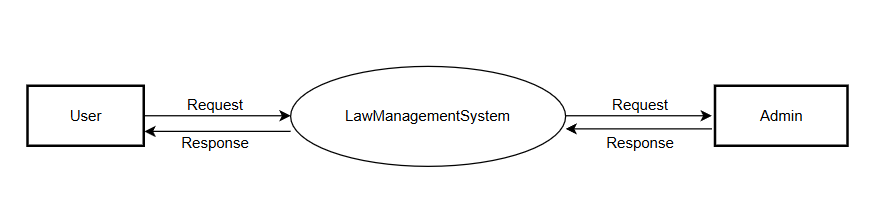
\includegraphics[width=0.8\linewidth]{LawDFD0.png}
 \caption{DFD LEVEL 0}
   \label{fig:DFD LEVEL 0}
\end{figure}


\begin{figure}
  \centering
  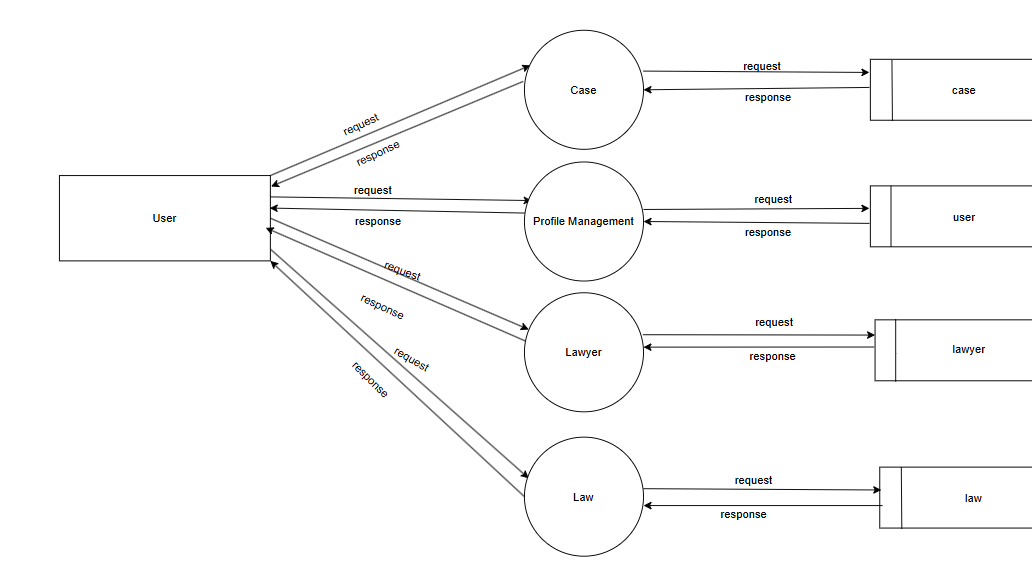
\includegraphics[width=0.8\linewidth]{LawDFD1User.png}
 \caption{DFD LEVEL 1 - User}
   \label{fig:DFD LEVEL 1 - User}
\end{figure}

\begin{figure}
  \centering
  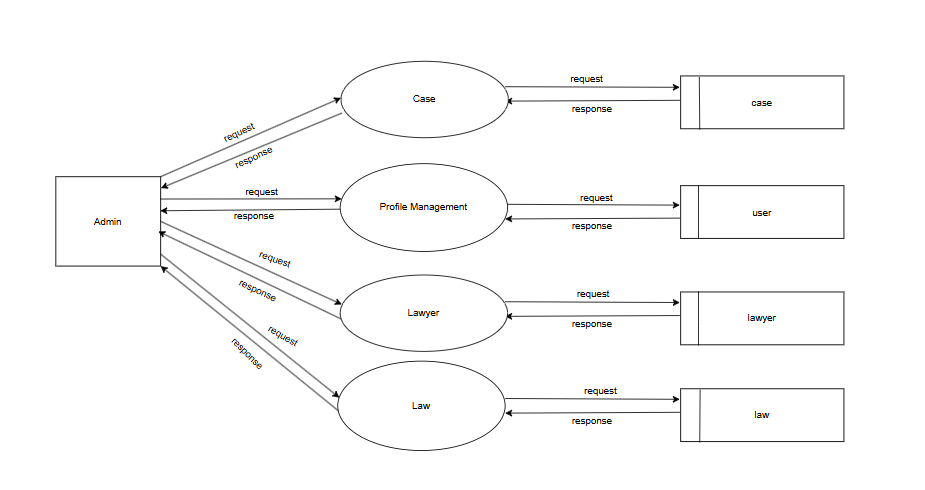
\includegraphics[width=0.8\linewidth]{LawDFD1Admin.png}
 \caption{DFD LEVEL 1 - Admin}
   \label{fig:DFD LEVEL 1 - Admin}
\end{figure}

\begin{figure}
  \centering
  \includegraphics[width=0.8\linewidth]{User2.1case.png}
 \caption{DFD LEVEL 2.1 - User}
   \label{fig:DFD LEVEL 2.1 - User}
\end{figure}

\begin{figure}
  \centering
  \includegraphics[width=0.8\linewidth]{User2.2user.png}
 \caption{DFD LEVEL 2.2- User}
   \label{fig:DFD LEVEL 2.2 - User}
\end{figure}

\begin{figure}
  \centering
  \includegraphics[width=0.8\linewidth]{User2.3lawyer.png}
 \caption{DFD LEVEL 2.3- User}
   \label{fig:DFD LEVEL 2.3 - User}
\end{figure}

\begin{figure}
  \centering
  \includegraphics[width=0.8\linewidth]{User2.4law.png}
 \caption{DFD LEVEL 2.4 - User}
   \label{fig:DFD LEVEL 2.4 - User}
\end{figure}

\begin{figure}
  \centering
  \includegraphics[width=0.8\linewidth]{Admin2.1case.png}
 \caption{DFD LEVEL 2.1 - Admin}
   \label{fig:DFD LEVEL 2.1 - Admin}
\end{figure}

\begin{figure}
  \centering
  \includegraphics[width=0.8\linewidth]{Admin2.2user.png}
 \caption{DFD LEVEL 2.2- Admin}
   \label{fig:DFD LEVEL 2.2 - Admin}
\end{figure}

\begin{figure}
  \centering
  \includegraphics[width=0.8\linewidth]{Admin2.3lawyer.png}
 \caption{DFD LEVEL 2.3- Admin}
   \label{fig:DFD LEVEL 2.3 - Admin}
\end{figure}

\begin{figure}
  \centering
  \includegraphics[width=0.8\linewidth]{Admin2.4law.png}
 \caption{DFD LEVEL 2.4 - Admin}
   \label{fig:DFD LEVEL 2.4 - Admin}
\end{figure}
%
\chapter{IMPLEMENTATION, TESTING AND VALIDATION}
%
\section{Implementation}

The "Law Management System" was implemented using Django, a powerful Python-based framework, which facilitated rapid development and secure data handling. The system comprises several modules, including authentication, case management, document management, and user management, each interacting with a centralized database. Role-based access was implemented to ensure data privacy and control user permissions, allowing admins, lawyers, and clients to access only their relevant information. Additionally, the database stores all legal records, case data, and documents securely, while the frontend interface is designed to be user-friendly and accessible from any device with an internet connection.
\section{Testing Methods}

Software testing methodologies are the various strategies or approaches used to test an application to ensure it behaves and looks as expected. These encompass everything from front to back-end testing, including unit and system testing.

\subsection{Unit Testing}

Unit testing focuses on verifying the smallest units of the application—usually individual functions or methods in the code. In the "Law Management System," unit tests would be created for core functionalities like user login, case creation, document upload, and data retrieval. Each unit test ensures that a specific part of the code works as expected in isolation, which helps identify bugs at an early stage. By testing individual components separately, developers can pinpoint errors and improve the reliability of the system. Unit tests are often automated, allowing developers to rerun them quickly after making code changes.

\subsection{Integration Testing}

Integration testing examines the interaction between different modules or components within the system. In the "Law Management System," this would involve testing how the case management module interacts with the document storage, or how user roles and permissions impact data access across various modules. The goal is to ensure that these components work together as intended and data flows correctly between them. Integration testing is essential for identifying issues that may arise when multiple components are combined, helping to ensure a smooth user experience and consistent data handling.

\subsection{System Testing}

System testing is conducted on the complete and integrated system to verify that it meets all specified requirements. This type of testing is performed from an end-user’s perspective, covering all functionalities within the "Law Management System," such as case registration, user management, document uploads, and role-based access. System testing ensures that the system behaves as expected in a production-like environment, simulating real-world scenarios. It’s a comprehensive test method that helps verify the overall functionality, reliability, and performance of the system before it is released.

\subsection{Acceptance Testing}

Acceptance testing is the final phase of testing, intended to determine whether the system meets the requirements and expectations of the end users. In the context of the "Law Management System," acceptance testing involves having real users (such as legal professionals and administrators) test the system to confirm that it functions according to their needs. This testing phase focuses on usability, accessibility, and real-world applicability, ensuring that the system is ready for deployment. Positive feedback from users in acceptance testing signifies that the system is ready to be deployed to a production environment.

\subsection{Regression Testing}

Regression testing is conducted to verify that recent changes or updates to the system (such as new features or bug fixes) have not introduced any new issues. In the "Law Management System," regression testing is essential after adding features like enhanced document management or updated case tracking functionalities. This test method involves rerunning previously executed test cases to ensure that existing functionality remains unaffected. By maintaining the stability of the system, regression testing helps provide a seamless user experience, even after regular updates or improvements.

\subsection{Usability Testing}

Usability testing focuses on assessing the user interface and overall user experience of the system. In the "Law Management System," usability testing would involve observing how legal professionals and clients navigate the system, view cases, upload documents, and access information. The goal is to identify any user interface issues, such as confusing navigation, unclear labels, or accessibility challenges. Feedback from usability testing helps refine the system’s design, ensuring that users can efficiently perform their tasks with minimal effort or frustration.
\section{Validation}
%	< Validation done in the project >
%
%   *********************  CHAPTER ***********************
To ensure the system meets all functional and security requirements, extensive validation and testing were conducted. Unit tests were implemented for each module to verify that individual functionalities—such as user authentication, case creation, and document uploads—operate correctly. Integration testing was conducted to confirm seamless data flow between modules. Role-based access was tested thoroughly to ensure that users can only access permitted sections and data. Finally, user acceptance testing involved gathering feedback from potential users to make sure the system met real-world needs and usability standards.
\chapter{CONCLUSION}
%
%   *********************  CHAPTER ***********************
The "Law Management System" successfully addresses the primary challenges faced by law firms in managing cases, documents, and client interactions. By digitizing and centralizing the management of legal processes, the system reduces paperwork, enhances data security, and improves operational efficiency. Legal professionals now have an effective tool to streamline case tracking, store documents securely, and communicate with clients seamlessly, all of which contributes to improved client satisfaction and productivity within law firms.
\chapter{SCOPE FOR FUTURE ENHANCEMENT}
%
%
%   *********************  CHAPTER ***********************
%
%%%%%%%%%%%%%%%%%%%%%%%%%  APPENDICES %%%%%%%%%%%%%%%%%%%%%
Future enhancements to the "Law Management System" could include advanced features like AI-based document analysis to assist in case preparation, a client portal for direct communication and appointment scheduling, and integration with external legal databases for case law research. Adding a mobile application could further improve accessibility for users on-the-go. Additionally, incorporating analytics and reporting tools could help law firms track case progress, workload distribution, and overall firm performance. These enhancements would make the system even more comprehensive, catering to a broader range of needs in the legal industry.
\clearpage
\addcontentsline{toc}{chapter}{APPENDICES}
\appendix
\quad\vfill
\begin{center}
{\Huge \bf APPENDICES}
\end{center}
\vfill
\clearpage
%
%
%   *********************  CHAPTER ***********************
%
%
\chapter{SCRUM PROCESS ARTIFACTS}
%
\section{Product Backlog}
%
% The following table is only a sample. 
%
\renewcommand{\arraystretch}{1.25}
\begin{center}
\begin{tabular}{|m{0.08\textwidth}|m{0.15\textwidth}|m{0.5\textwidth}|m{0.1\textwidth}|}
\hline
{\bf Priority} & {\bf Product backlog items} & {\bf User story} & {\bf Estimate (Hours)}\\
\hline
1 & Database creation & As an operations engineer, I want to be able to store all customer information.  & 240 \\
\hline
2 & Login page & As a site member I want to login to the site. & 160 \\
\hline
3 & Category page & As a site member, I want to be able to look for different categories of brands. & 400\\
\hline
4 & Payment process & As a site member, I want to be able to make payments. & 240\\
\hline
5 & Contact page & As a site member, I want to be able to find contact information of the site. & 80 \\
\hline
6 & Banner area & As a marketing personnel, I want to be able to make advertisement. & 40\\
\hline
\end{tabular}
\end{center}
%
\section{Scrum Meeting Details}
%
\begin{center}
\begin{tabular}{|m{0.03\textwidth}|m{0.05\textwidth}|m{0.3\textwidth}|m{0.2\textwidth}|m{0.2\textwidth}|}
\hline
Sl. No. & Date & Sprint backlog & Product shippable Increment & Important Decisions \\
\hline
& & & &  \\
\hline
\end{tabular}
\end{center}

\renewcommand{\arraystretch}{1}
%
%   *********************  APPENDIX ***********************
%
\chapter{DIAGRAMS}
\section{Entity Relationship Diagram}
\begin{figure}
  \centering
  \includegraphics[width=1\linewidth]{ERLAW.png}
 \caption{ER Diagram}
   \label{fig:ER-diagram}
\end{figure}
%
%
%   *********************  APPENDIX ***********************
%
\chapter{TABLE STRUCTURE}
%----------------------------------------------------------------------------------------------------------------------
%❗❗❗❗❗❗❗❗user table
\begin{table}[h]
   \centering
    \begin{tabular}{|l|l|l|l|l|}
    \hline 
    Sl. No.&  Field&  Datatype&  Constraint& Description \\
     \hline  
      1& user\_id &int  &primary key  &To store User id \\ 
      \hline 
      2&username  &varchar  &not null  &To store User name  \\
      \hline 
        3& email &varchar  &not null  &To store User email \\
   \hline
        4& password &varchar  &not null  &To store User password \\

\hline
    \end{tabular}
\caption{User}
\label{tab:User}
\end{table}
%----------------------------------------------------------------------------------------------------------------------
%❗❗❗❗❗❗❗❗-Law table-----------------
\begin{table}[h]
   \centering
    \begin{tabular}{|l|l|l|l|l|}
    \hline 
    Sl. No.&  Field&  Datatype&  Constraint& Description \\
     \hline  
      1& law\_id &int  &primary key  &To store Law id \\ 
      \hline 
      2&law\_title  &varchar  &not null  &To store Law  \\
      \hline 
        3& law\_act &varchar  &not null  &To store Law act \\
   \hline 
        4& law\_category &varchar  &not null  &To store Lawy category \\
   \hline
        5& law\_description &varchar  &not null  &To store Law description \\


\hline
    \end{tabular}
\caption{Law }
\label{tab:Law}
\end{table}
%----------------------------------------------------------------------------------------------------------------------
%❗❗❗❗❗❗❗❗-Lawyer table-----------------
\begin{table}[h]
   \centering
    \begin{tabular}{|l|l|l|l|l|}
    \hline 
    Sl. No.&  Field&  Datatype&  Constraint& Description \\
     \hline  
      1& lawyer\_id &int  &primary key  &To store Lawyer id \\ 
      \hline 
      2&image  &imagefield  &not null  &To store Lawyer image  \\
      \hline 
        3& name &varchar  &not null  &To store Lawyer name \\
   \hline 
        4& section &varchar  &not null  &To store Lawyer section \\
   \hline
        5& experience &int  &not null  &To store Lawyer experience \\
   \hline
        6& fees &int  &not null  &To store Lawyer fess \\
 
\hline
    \end{tabular}
\caption{Lawyer}
\label{tab:Lawyer}
\end{table}
%----------------------------------------------------------------------------------------------------------------------
%❗❗❗❗❗❗❗❗Case Table-----------------
\begin{table}[h]
   \centering
    \begin{tabular}{|l|l|l|l|l|}
    \hline 
    Sl. No.&  Field&  Datatype&  Constraint& Description \\
     \hline  
      1& case\_id &int  &primary key  &To store Case id \\ 
      \hline 
      2&case\_title  &varchar  &not null  &To store Case title  \\
      \hline 
        3& petitioner\_name &varchar  &not null  &To store Petitioner name \\
   \hline 
        4& petitioner\_phone &varchar  &not null  &To store Petitioner phone number \\
   \hline
        5& petitioner\_email &varchar  &not null  &To store Petitioner email address \\
   \hline
        6& petitioner\_address &varchar  &not null  &To store Petitioner  address \\
   \hline
        7& petitioner\_district &varchar  &not null  &To store Petitioner  district \\
   \hline
        8& court &varchar  &not null  &To store Petitioner case appealing court \\
   \hline
        9& case\_date &date  &not null  &To store Petitioner case date \\
   \hline
        10& case\_describtion &varchar  &not null  &To store Petitioner case describtion \\
   \hline
        11& is\_approved &boolean  &not null  &To store Case Status \\

\hline
    \end{tabular}
\caption{Case}
\label{tab:Case}
\end{table}

%   *********************  APPENDIX ***********************
%
\chapter{SAMPLE SCREENSHOTS}
\begin{figure}
  \centering
  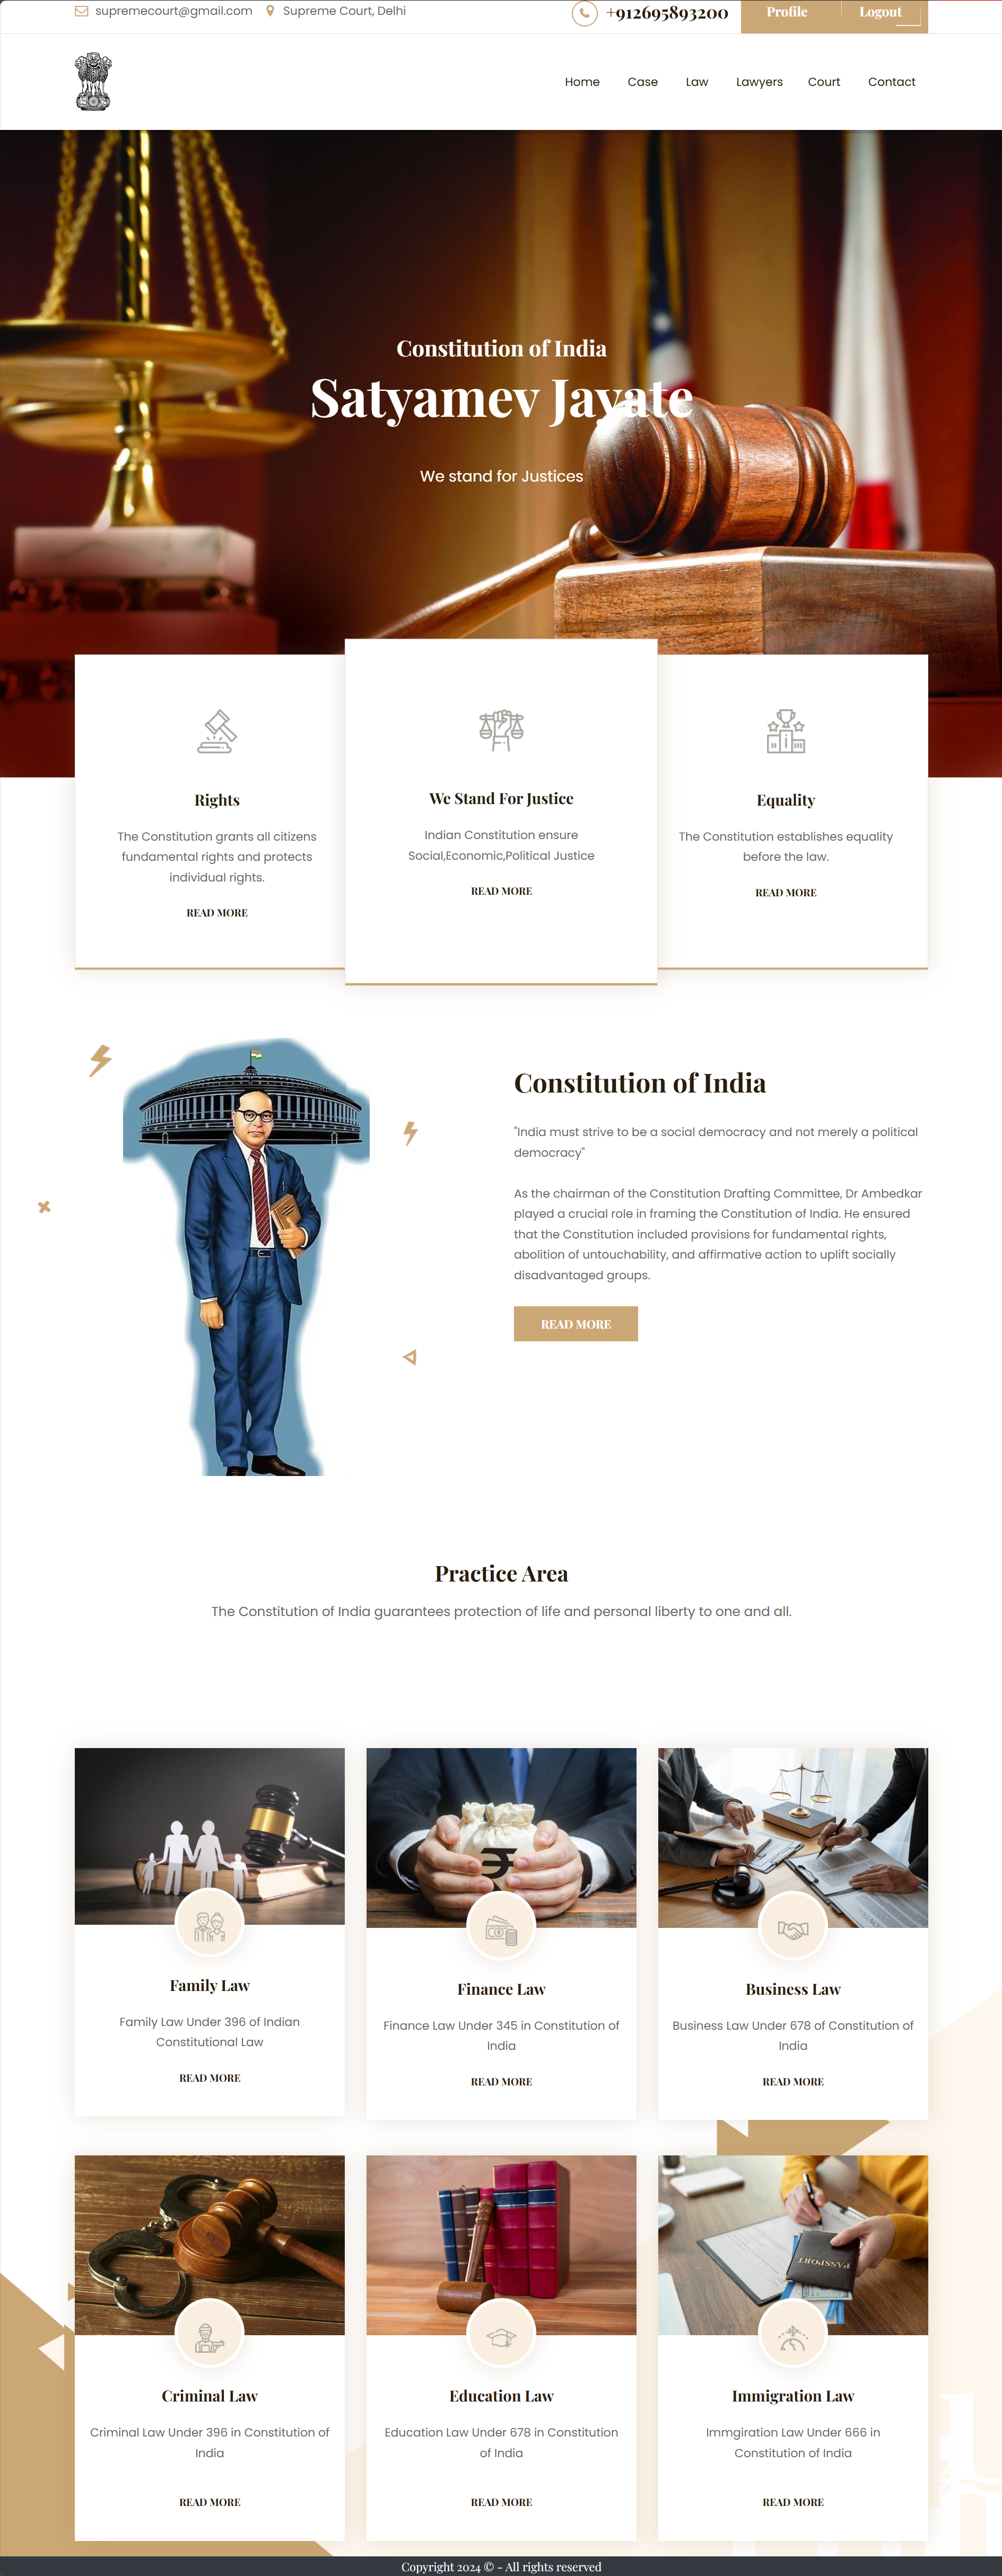
\includegraphics[width=0.5\linewidth]{indexpage.png}
 \caption{Index page}
   \label{fig:Index page}
\end{figure}

\begin{figure}
  \centering
  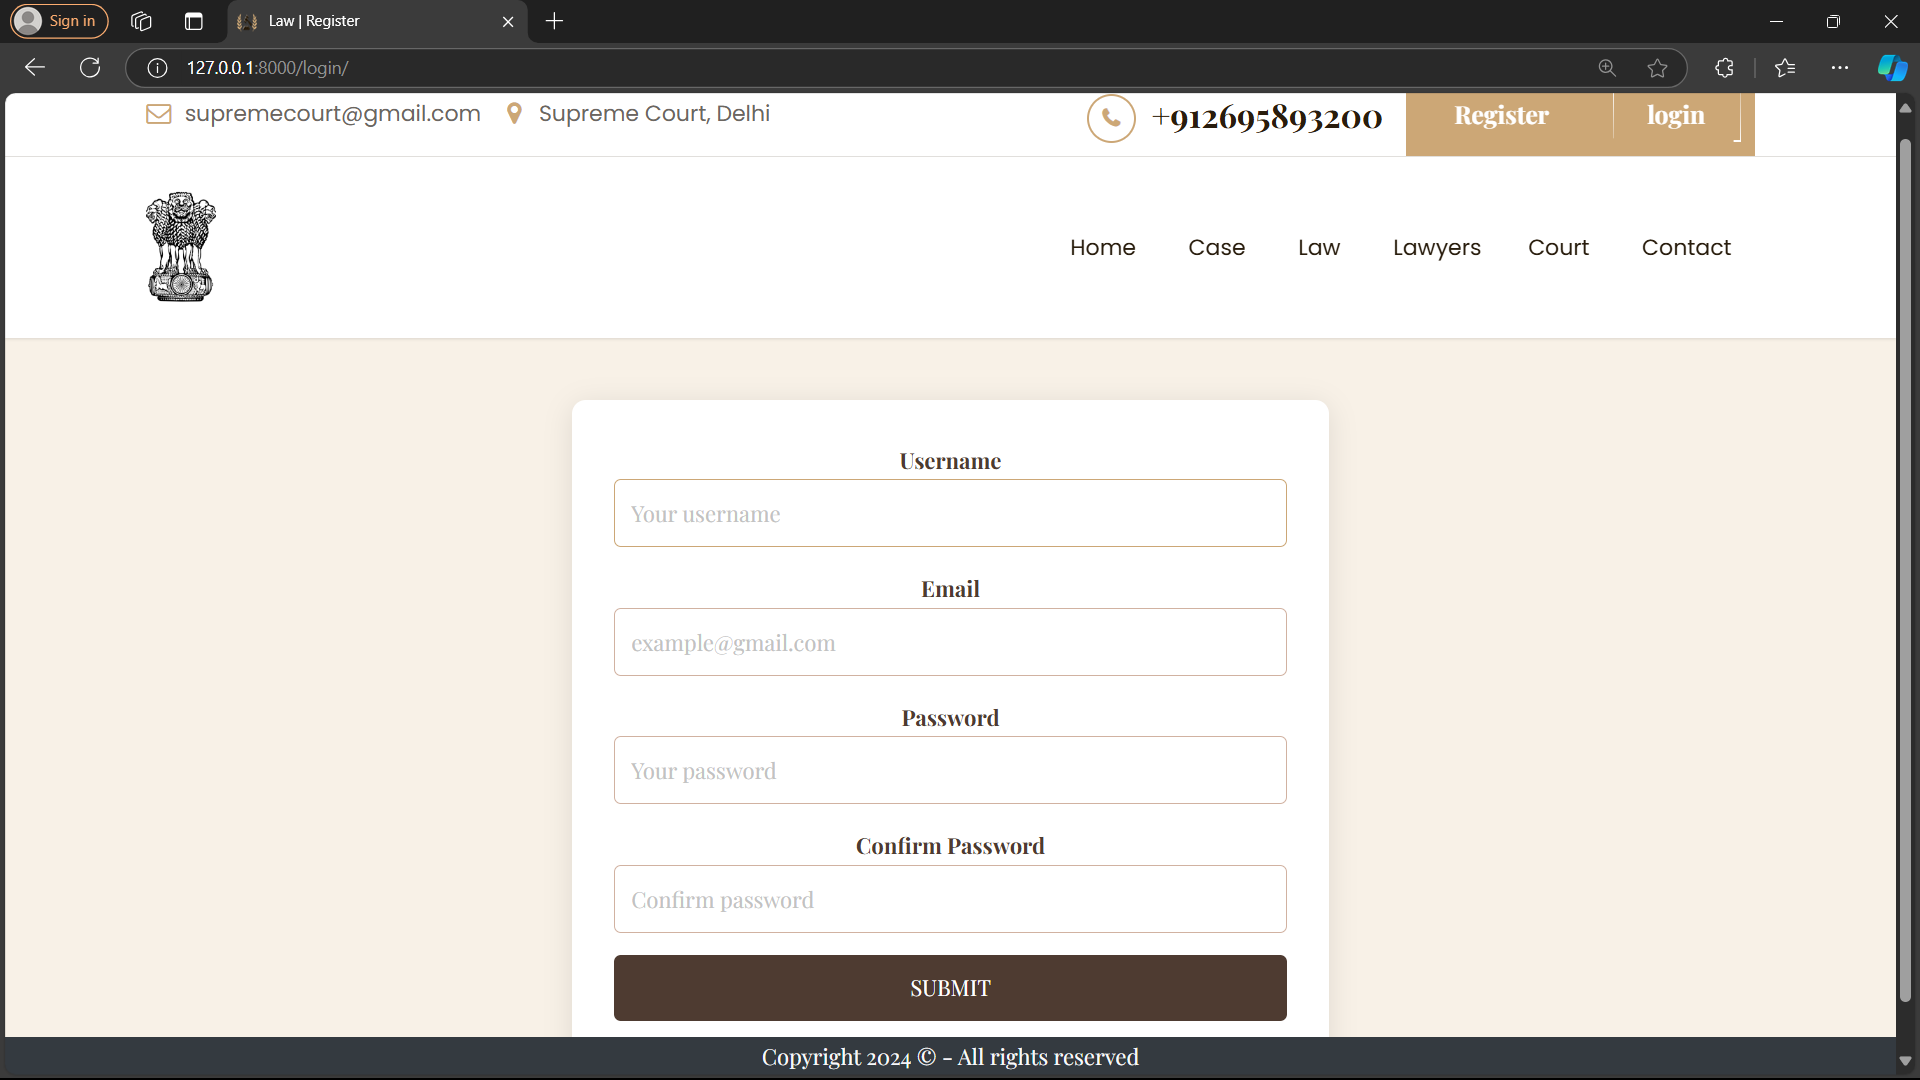
\includegraphics[width=0.5\linewidth]{registration.png}
 \caption{User Registration}
   \label{fig:User Registration}
\end{figure}

\begin{figure}
  \centering
  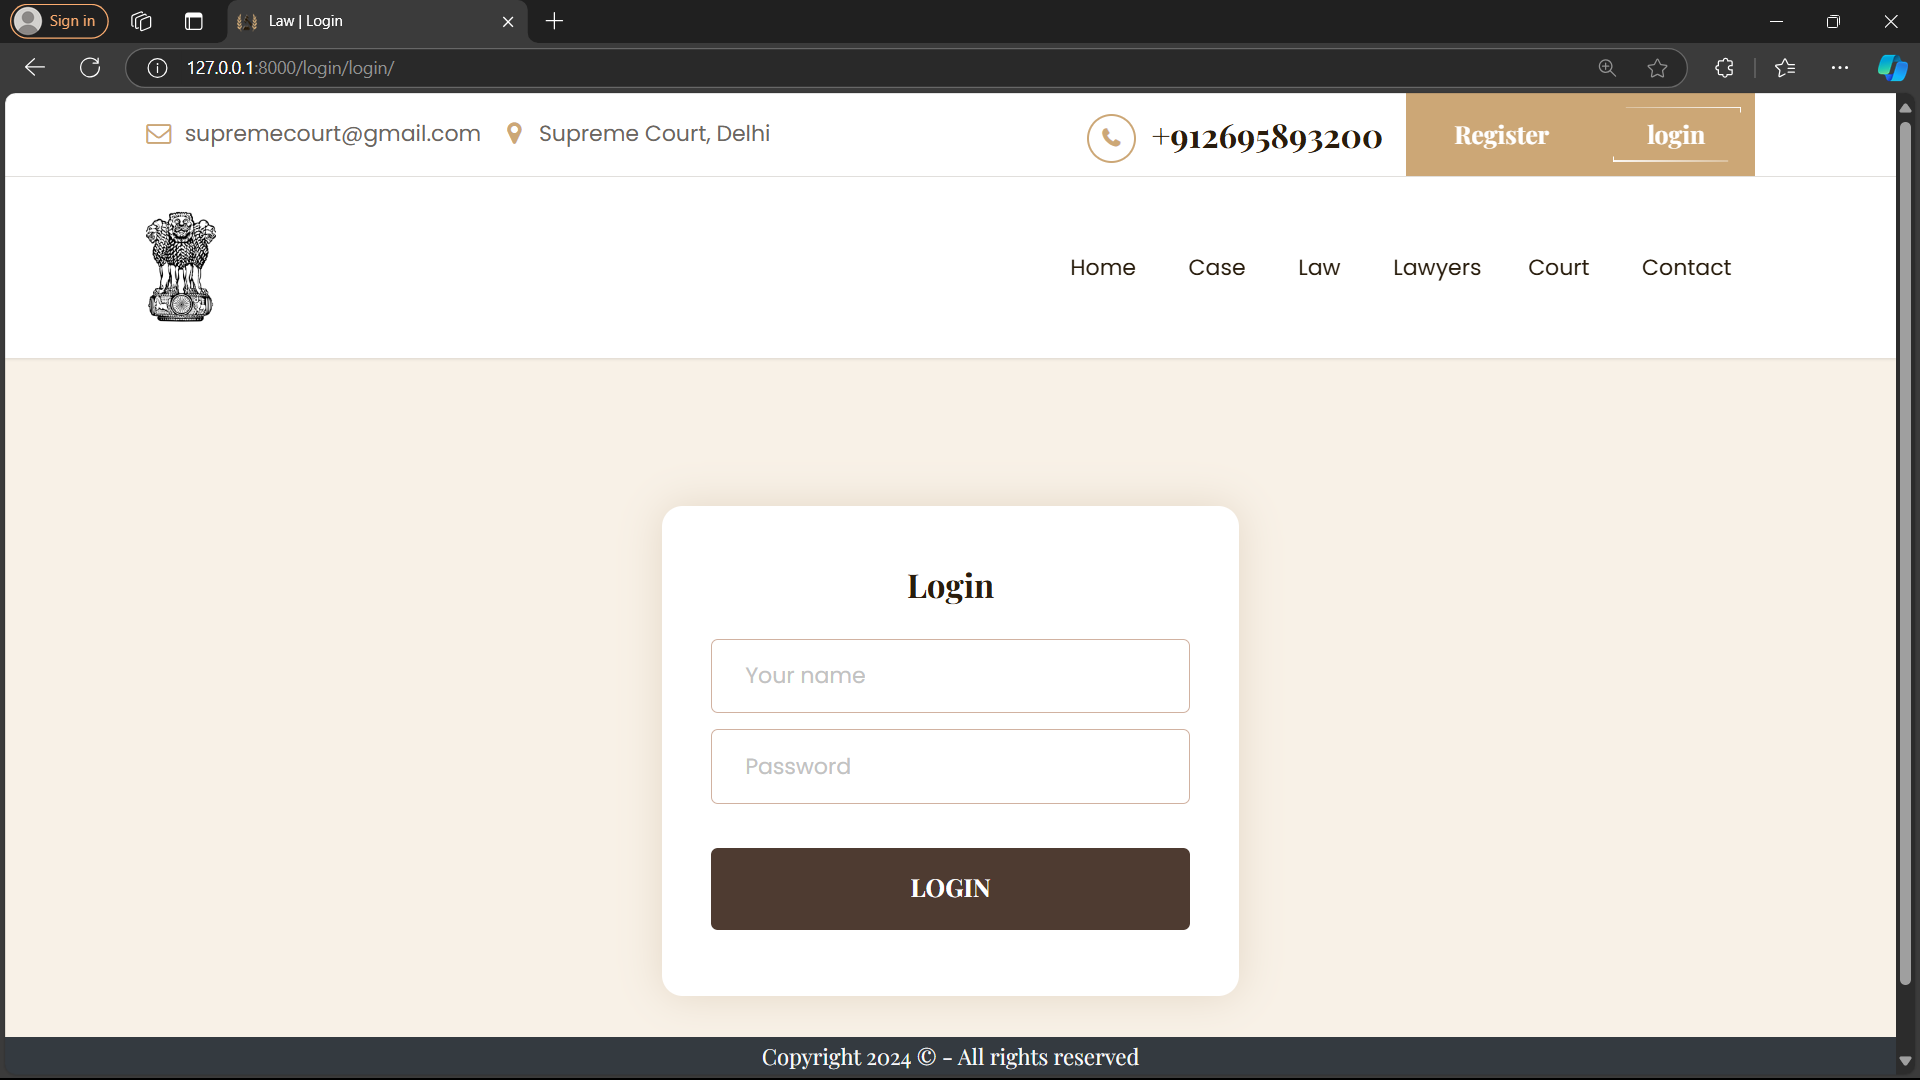
\includegraphics[width=0.5\linewidth]{login.png}
 \caption{User Login}
   \label{fig:User Login}
\end{figure}

\begin{figure}
  \centering
  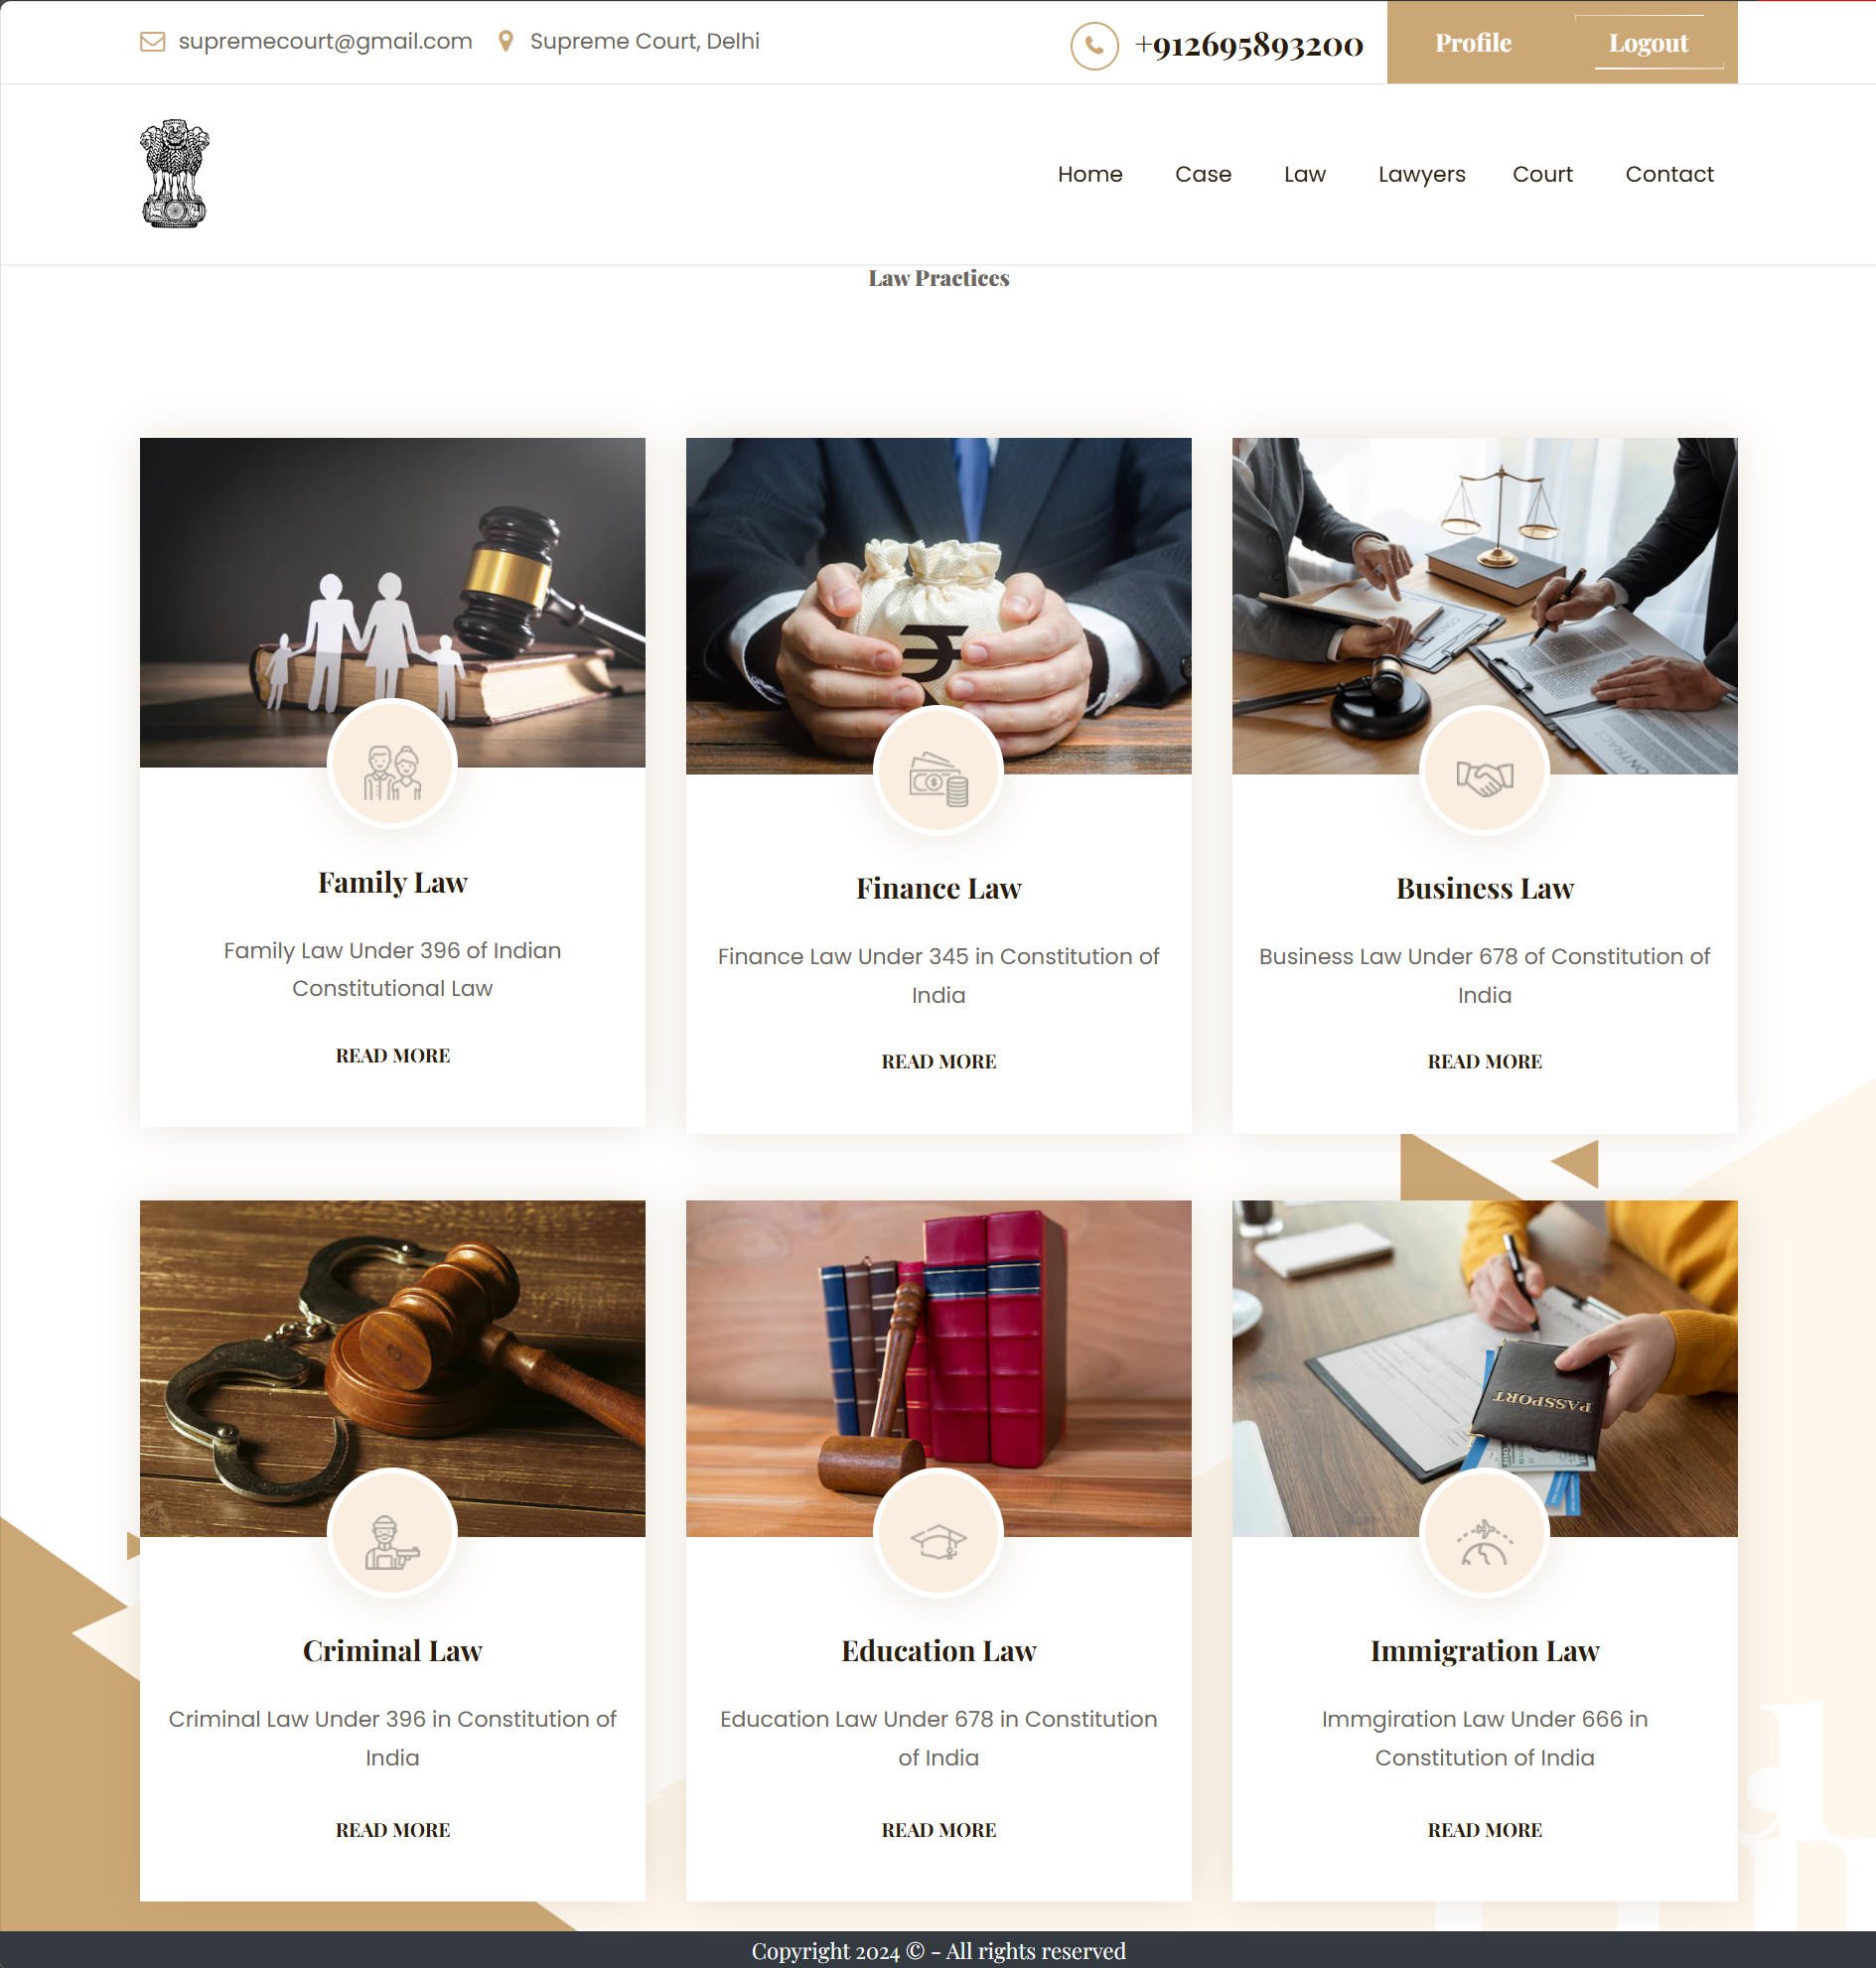
\includegraphics[width=0.5\linewidth]{lawpage.png}
 \caption{Law Page}
   \label{fig:Law Page}
\end{figure}

\begin{figure}
  \centering
  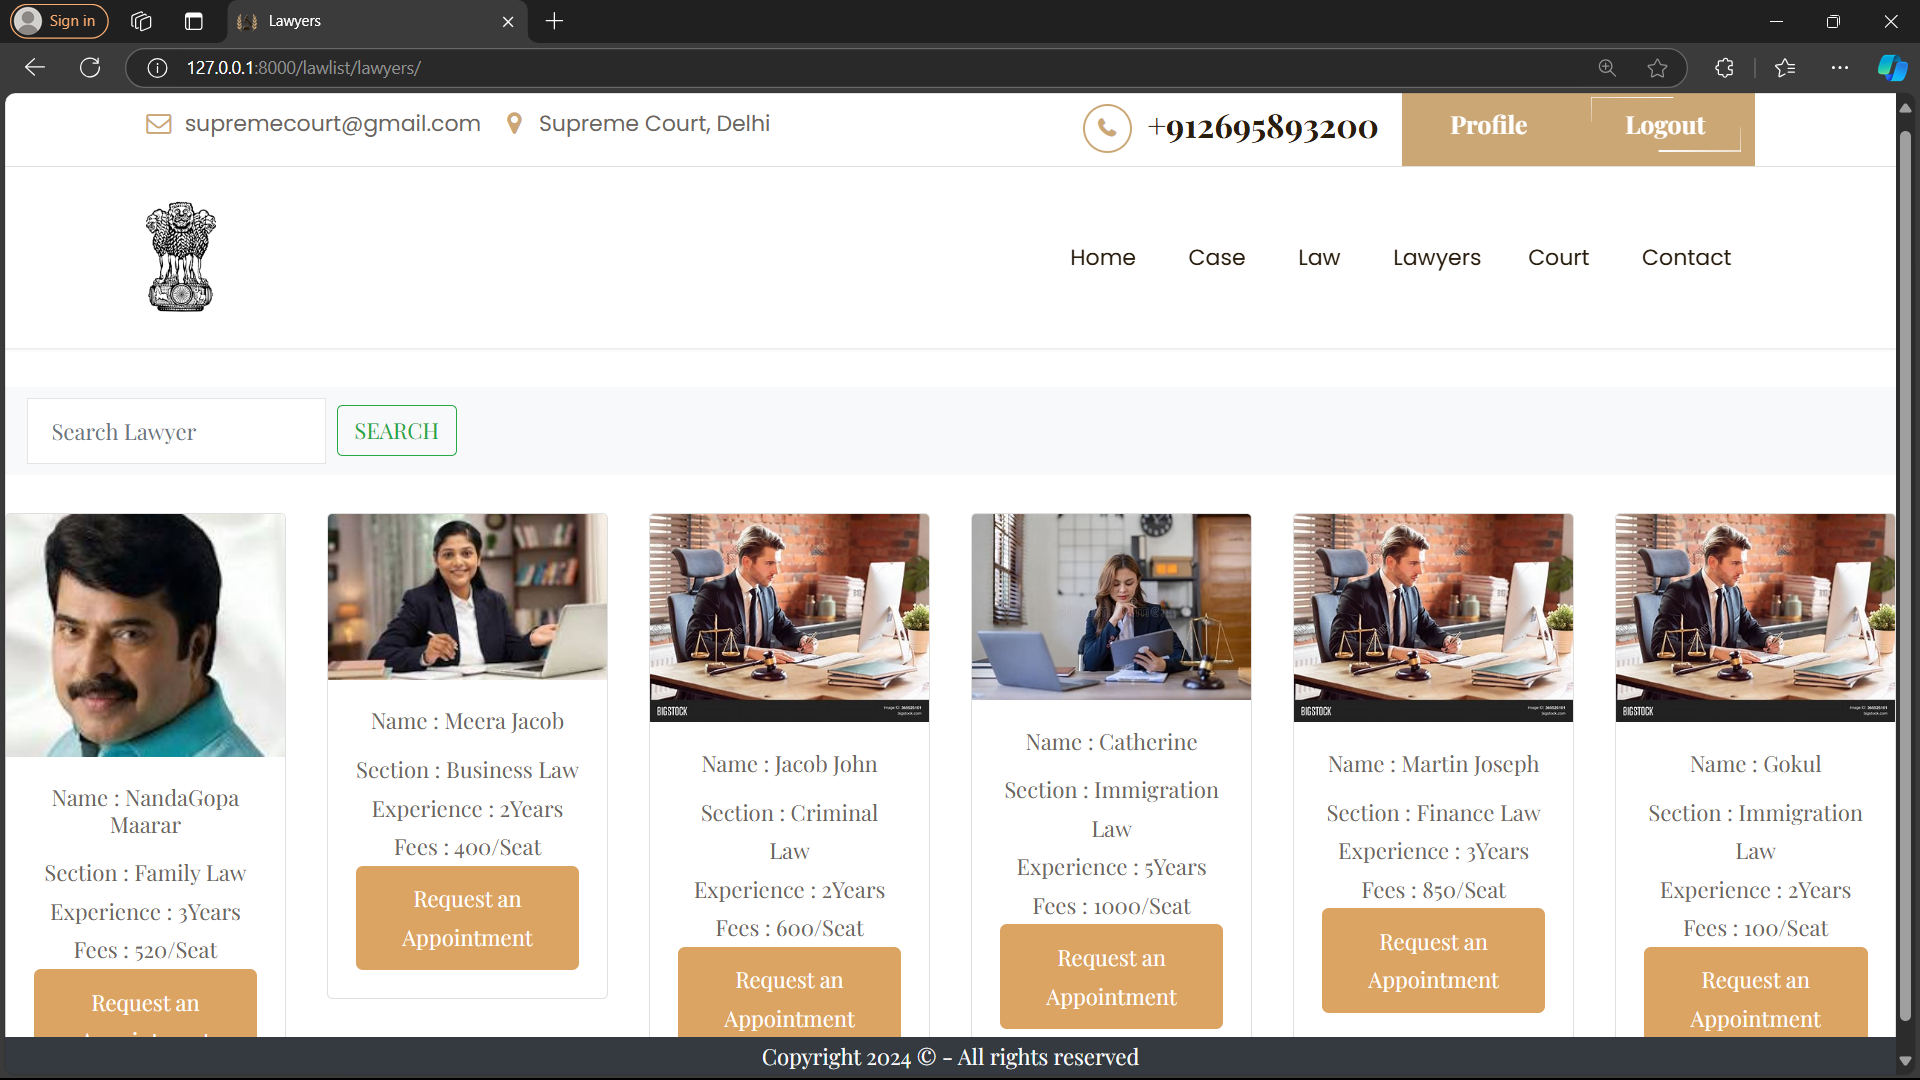
\includegraphics[width=0.5\linewidth]{lawyers.png}
 \caption{Lawyer Page}
   \label{fig:Lawyer Page}
\end{figure}

\begin{figure}
  \centering
  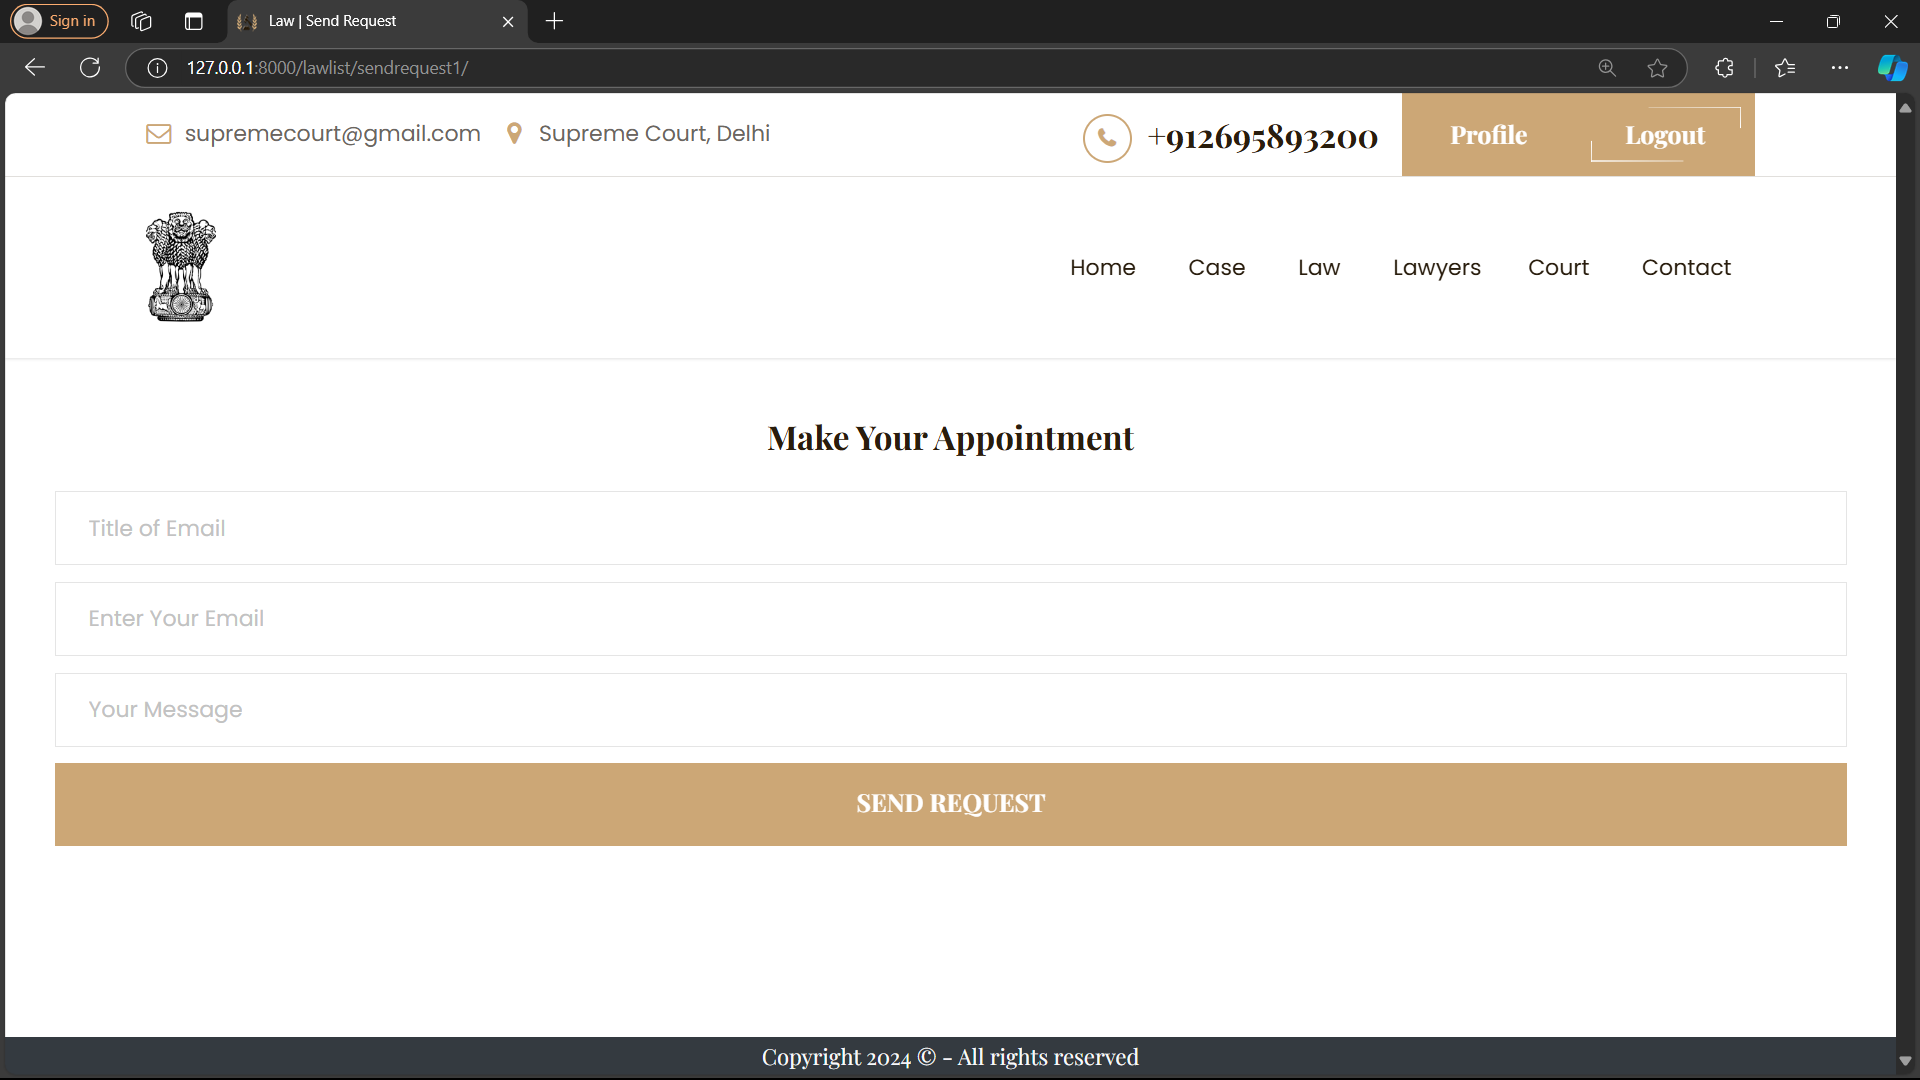
\includegraphics[width=0.5\linewidth]{sendrequest.png}
 \caption{Send Appointment Request}
   \label{fig:Send Appointment Request}
\end{figure}

\begin{figure}
  \centering
  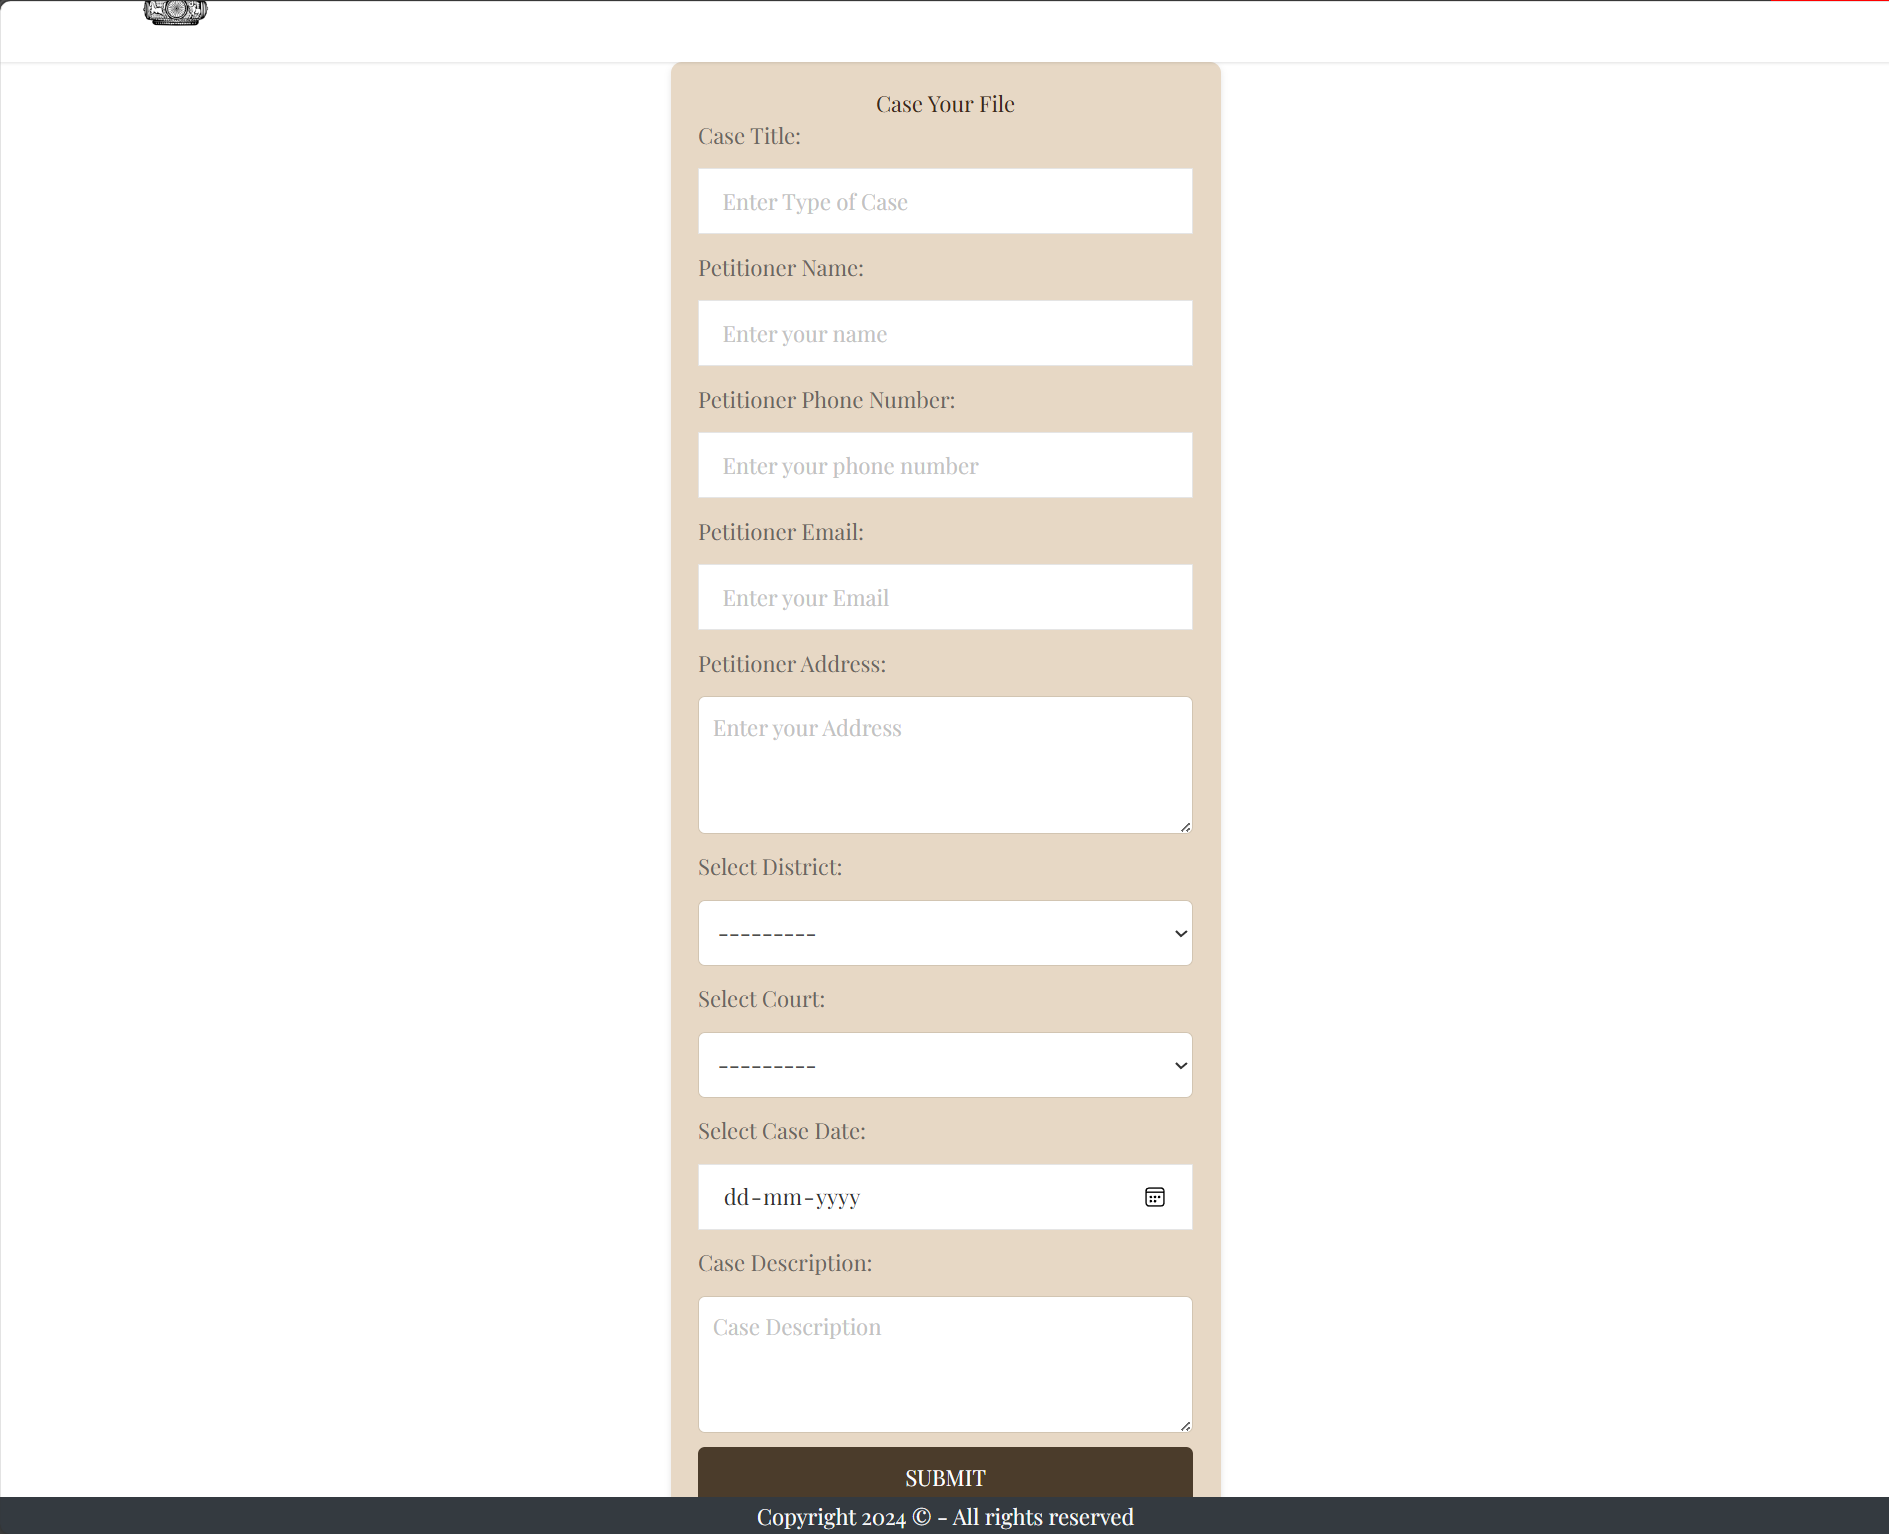
\includegraphics[width=0.5\linewidth]{caseuploadpage.png}
 \caption{Case Upload Page}
   \label{fig:Case Upload Page}
\end{figure}

\begin{figure}
  \centering
  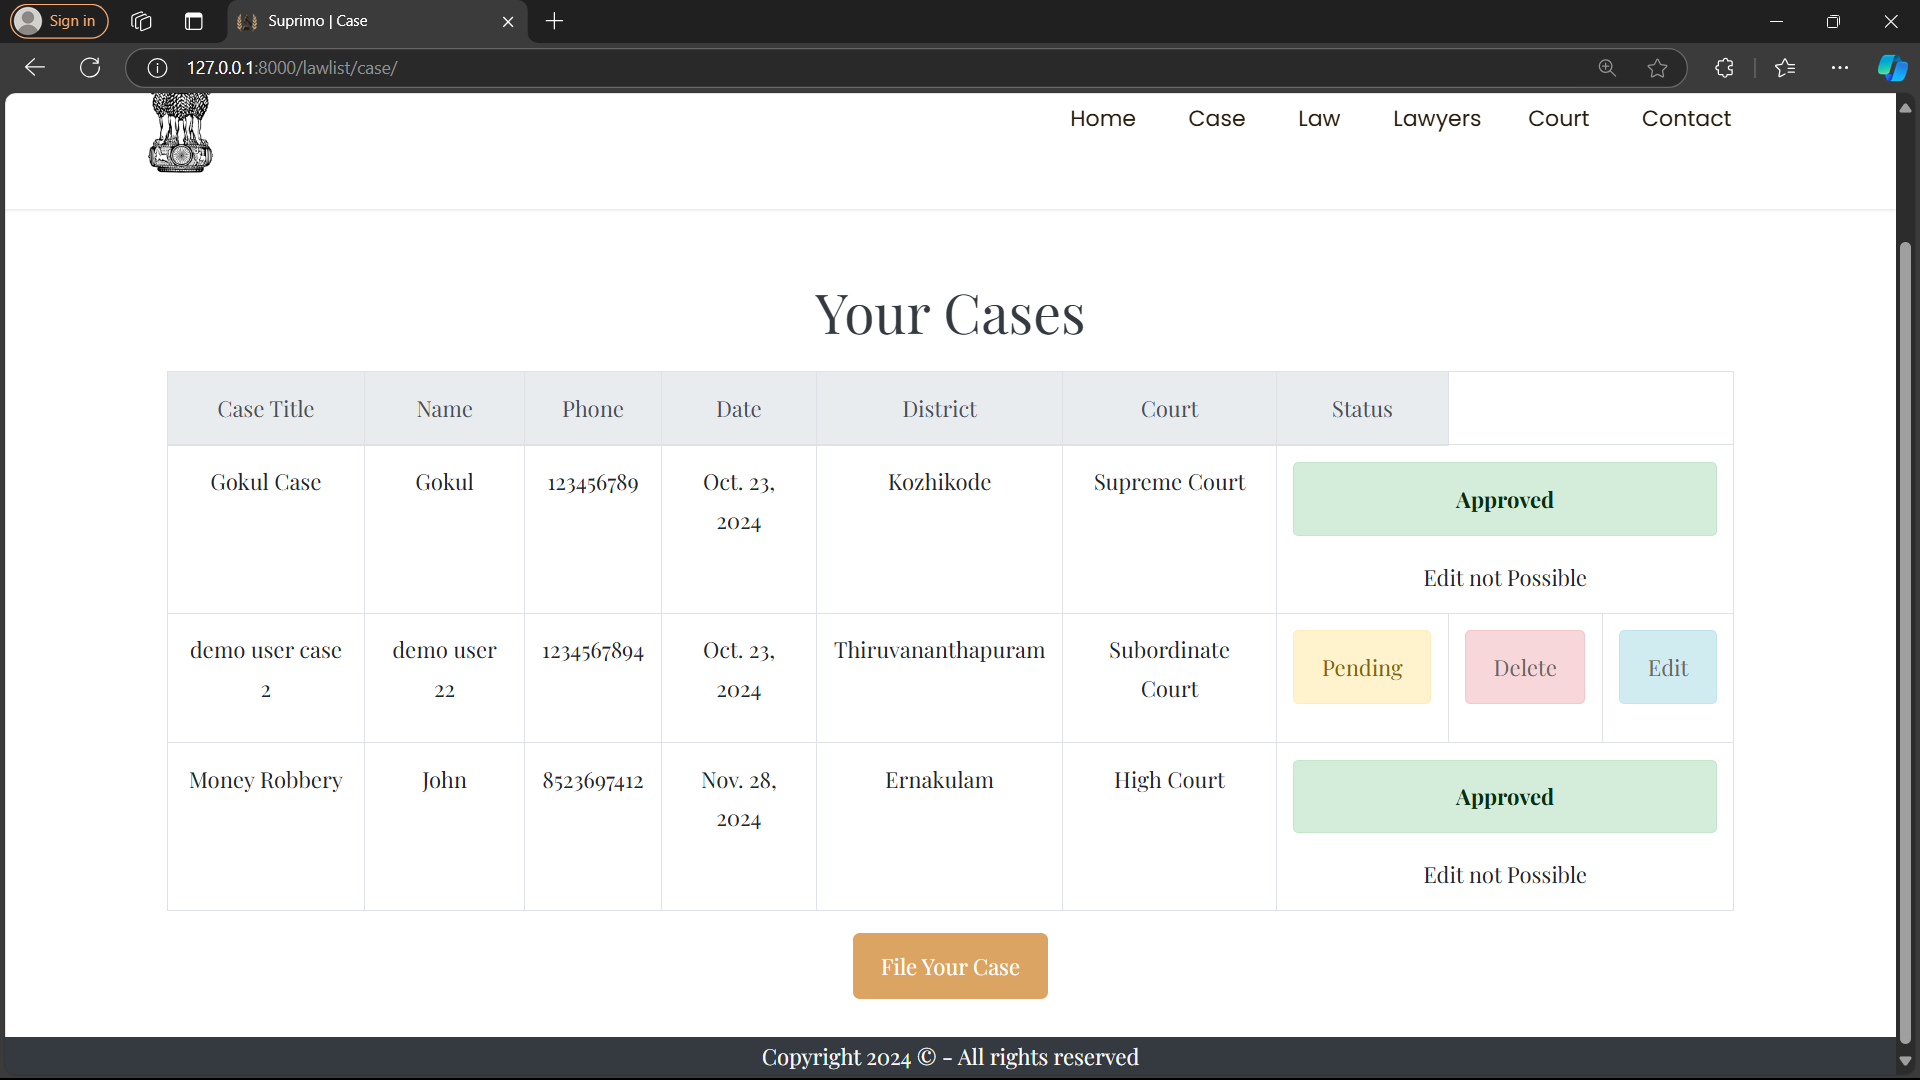
\includegraphics[width=0.5\linewidth]{uploadedcases.png}
 \caption{User Cases}
   \label{fig:User Cases}
\end{figure}

\begin{figure}
  \centering
  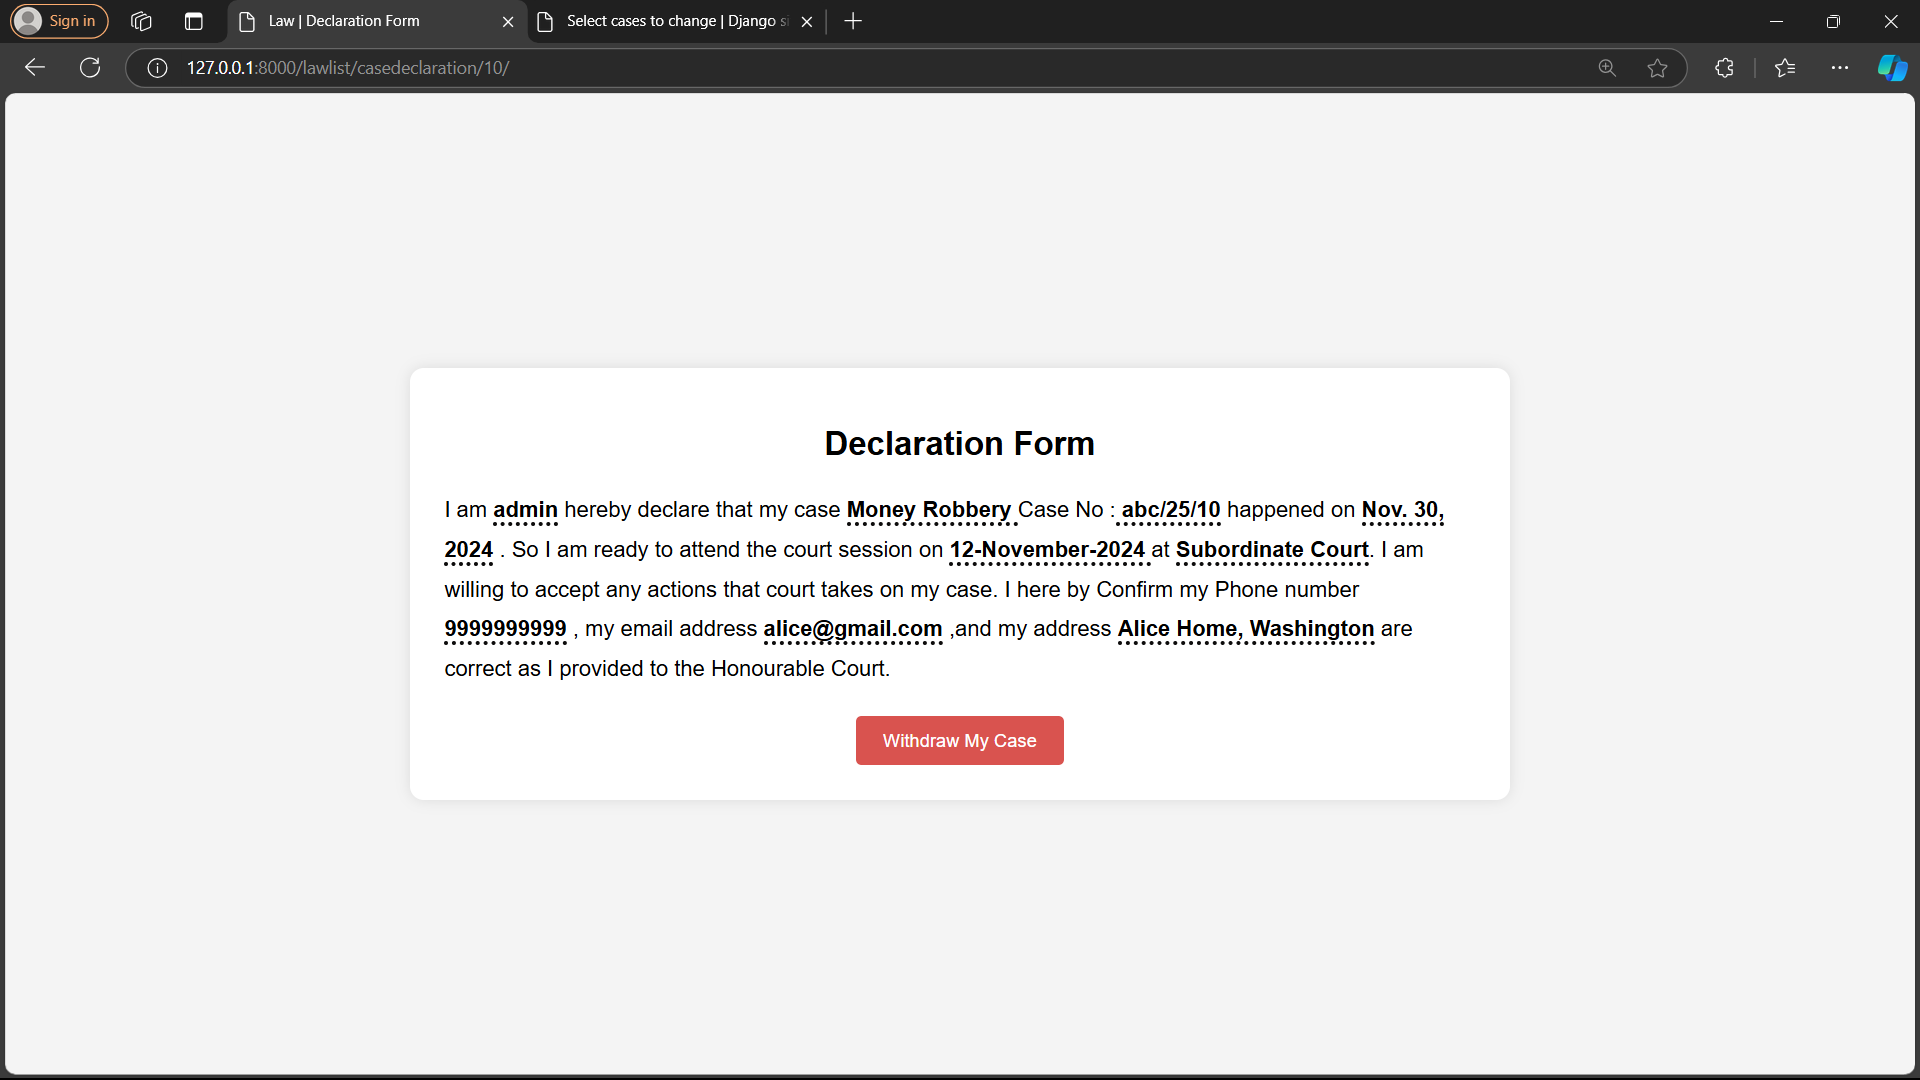
\includegraphics[width=0.5\linewidth]{casereport.png}
 \caption{Case Report}
   \label{fig:Case Report}
\end{figure}

\begin{figure}
  \centering
  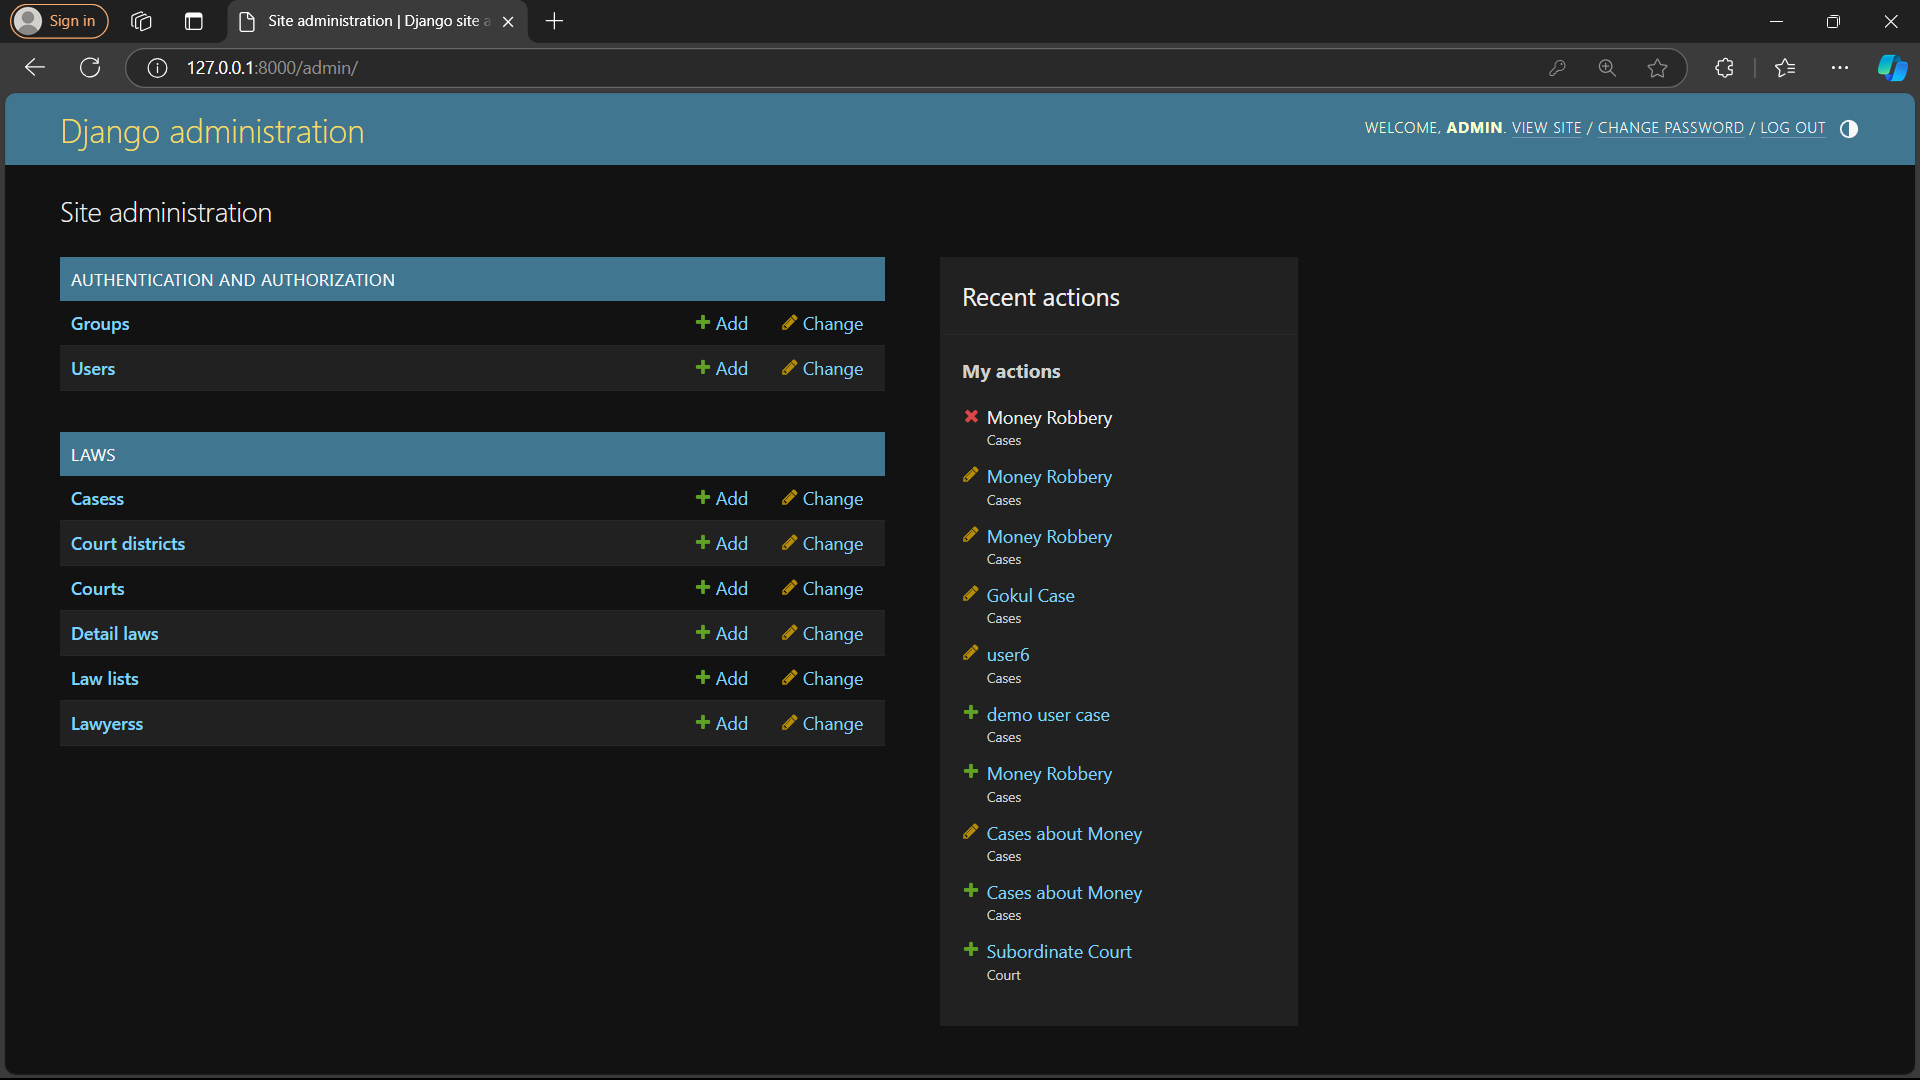
\includegraphics[width=0.5\linewidth]{adminpage.png}
 \caption{Admin Page}
   \label{fig:Admin Page}
\end{figure}

%
% ***   Creating Bibliography   ***
%
% Do not delete the following two lines
%
\clearpage
\addcontentsline{toc}{chapter}{Bibliography}
%
%   The markups for creating the bibliography 
%   begins here. Do not change the two lines 
%   "\begin{thebibliography}{99}" and 
%   "\end{thebibliography}".
%   One sample bibliography item is included. 
%   Each new item is to be preceded by
%   "\bibitem{itemx}".
%   Add additional items if there are any.
%   Bibliography styles:
%   Titles of books   : Italics  {use {\em Title} )
%   URLs of websites  : Type-writer (use {\tt Title} )
%   Titles of papers  : In double quotes (use ``Title")
%
\begin{thebibliography}{99}
%
\bibitem{item1}
{\em First Lessons in \LaTeX}, by Dr. V N Krishnachandran, 
Vidya Academy of Science \& Technology, 
Thrissur - 680 501, 2011.
%
\end{thebibliography}
%
%
%   Printing the last page
%
%
\newpage
\thispagestyle{empty}
\vspace*{\fill}
\begin{flushright}

\includegraphics{VidyaLogo}\\[0.5cm]
{\Large \bf \sf  Department of \vdept\ }\\
{\sf Vidya Academy of Science \& Technology\\
Thalakkottukara, Thrissur - 680 501\\
({\tt http://www.vidyaacademy.ac.in})}
\end{flushright}
%
%
%
%   ***   The end   ***
%
%
\end{document}